\documentclass[]{elsarticle} %review=doublespace preprint=single 5p=2 column
%DIF LATEXDIFF DIFFERENCE FILE
%DIF DEL Bike-share-spatial-equity-R1.tex   Mon Aug 30 16:30:52 2021
%DIF ADD Bike-share-spatial-equity.tex      Mon Aug 30 16:42:31 2021
%%% Begin My package additions %%%%%%%%%%%%%%%%%%%
\usepackage[hyphens]{url}

  \journal{Transportation Research Part D: Transport and
Environment} % Sets Journal name


\usepackage{lineno} % add
\providecommand{\tightlist}{%
  \setlength{\itemsep}{0pt}\setlength{\parskip}{0pt}}

\usepackage{graphicx}
\usepackage{booktabs} % book-quality tables
%%%%%%%%%%%%%%%% end my additions to header

\usepackage[T1]{fontenc}
\usepackage{lmodern}
\usepackage{amssymb,amsmath}
\usepackage{ifxetex,ifluatex}
\usepackage{fixltx2e} % provides \textsubscript
% use upquote if available, for straight quotes in verbatim environments
\IfFileExists{upquote.sty}{\usepackage{upquote}}{}
\ifnum 0\ifxetex 1\fi\ifluatex 1\fi=0 % if pdftex
  \usepackage[utf8]{inputenc}
\else % if luatex or xelatex
  \usepackage{fontspec}
  \ifxetex
    \usepackage{xltxtra,xunicode}
  \fi
  \defaultfontfeatures{Mapping=tex-text,Scale=MatchLowercase}
  \newcommand{\euro}{€}
\fi
% use microtype if available
\IfFileExists{microtype.sty}{\usepackage{microtype}}{}
\bibliographystyle{elsarticle-harv}
\ifxetex
  \usepackage[setpagesize=false, % page size defined by xetex
              unicode=false, % unicode breaks when used with xetex
              xetex]{hyperref}
\else
  \usepackage[unicode=true]{hyperref}
\fi
\hypersetup{breaklinks=true,
            bookmarks=true,
            pdfauthor={},
            pdftitle={Examining equity in accessibility to bike share: a balanced floating catchment area approach},
            colorlinks=false,
            urlcolor=blue,
            linkcolor=magenta,
            pdfborder={0 0 0}}
\urlstyle{same}  % don't use monospace font for urls

\setcounter{secnumdepth}{0}
% Pandoc toggle for numbering sections (defaults to be off)
\setcounter{secnumdepth}{0}

% Pandoc citation processing
\newlength{\cslhangindent}
\setlength{\cslhangindent}{1.5em}
\newlength{\csllabelwidth}
\setlength{\csllabelwidth}{3em}
% for Pandoc 2.8 to 2.10.1
\newenvironment{cslreferences}%
  {}%
  {\par}
% For Pandoc 2.11+
\newenvironment{CSLReferences}[2] % #1 hanging-ident, #2 entry spacing
 {% don't indent paragraphs
  \setlength{\parindent}{0pt}
  % turn on hanging indent if param 1 is 1
  \ifodd #1 \everypar{\setlength{\hangindent}{\cslhangindent}}\ignorespaces\fi
  % set entry spacing
  \ifnum #2 > 0
  \setlength{\parskip}{#2\baselineskip}
  \fi
 }%
 {}
\usepackage{calc}
\newcommand{\CSLBlock}[1]{#1\hfill\break}
\newcommand{\CSLLeftMargin}[1]{\parbox[t]{\csllabelwidth}{#1}}
\newcommand{\CSLRightInline}[1]{\parbox[t]{\linewidth - \csllabelwidth}{#1}\break}
\newcommand{\CSLIndent}[1]{\hspace{\cslhangindent}#1}

% Pandoc header
\usepackage{setspace}\doublespacing
\usepackage{booktabs}
\usepackage{longtable}
\usepackage{array}
\usepackage{multirow}
\usepackage{wrapfig}
\usepackage{float}
\usepackage{colortbl}
\usepackage{pdflscape}
\usepackage{tabu}
\usepackage{threeparttable}
\usepackage{threeparttablex}
\usepackage[normalem]{ulem}
\usepackage{makecell}
\usepackage{xcolor}
%DIF PREAMBLE EXTENSION ADDED BY LATEXDIFF
%DIF UNDERLINE PREAMBLE %DIF PREAMBLE
\RequirePackage[normalem]{ulem} %DIF PREAMBLE
\RequirePackage{color}\definecolor{RED}{rgb}{1,0,0}\definecolor{BLUE}{rgb}{0,0,1} %DIF PREAMBLE
\providecommand{\DIFaddtex}[1]{{\protect\color{blue}\uwave{#1}}} %DIF PREAMBLE
\providecommand{\DIFdeltex}[1]{{\protect\color{red}\sout{#1}}}                      %DIF PREAMBLE
%DIF SAFE PREAMBLE %DIF PREAMBLE
\providecommand{\DIFaddbegin}{} %DIF PREAMBLE
\providecommand{\DIFaddend}{} %DIF PREAMBLE
\providecommand{\DIFdelbegin}{} %DIF PREAMBLE
\providecommand{\DIFdelend}{} %DIF PREAMBLE
\providecommand{\DIFmodbegin}{} %DIF PREAMBLE
\providecommand{\DIFmodend}{} %DIF PREAMBLE
%DIF FLOATSAFE PREAMBLE %DIF PREAMBLE
\providecommand{\DIFaddFL}[1]{\DIFadd{#1}} %DIF PREAMBLE
\providecommand{\DIFdelFL}[1]{\DIFdel{#1}} %DIF PREAMBLE
\providecommand{\DIFaddbeginFL}{} %DIF PREAMBLE
\providecommand{\DIFaddendFL}{} %DIF PREAMBLE
\providecommand{\DIFdelbeginFL}{} %DIF PREAMBLE
\providecommand{\DIFdelendFL}{} %DIF PREAMBLE
%DIF HYPERREF PREAMBLE %DIF PREAMBLE
\providecommand{\DIFadd}[1]{\texorpdfstring{\DIFaddtex{#1}}{#1}} %DIF PREAMBLE
\providecommand{\DIFdel}[1]{\texorpdfstring{\DIFdeltex{#1}}{}} %DIF PREAMBLE
\newcommand{\DIFscaledelfig}{0.5}
%DIF HIGHLIGHTGRAPHICS PREAMBLE %DIF PREAMBLE
\RequirePackage{settobox} %DIF PREAMBLE
\RequirePackage{letltxmacro} %DIF PREAMBLE
\newsavebox{\DIFdelgraphicsbox} %DIF PREAMBLE
\newlength{\DIFdelgraphicswidth} %DIF PREAMBLE
\newlength{\DIFdelgraphicsheight} %DIF PREAMBLE
% store original definition of \includegraphics %DIF PREAMBLE
\LetLtxMacro{\DIFOincludegraphics}{\includegraphics} %DIF PREAMBLE
\newcommand{\DIFaddincludegraphics}[2][]{{\color{blue}\fbox{\DIFOincludegraphics[#1]{#2}}}} %DIF PREAMBLE
\newcommand{\DIFdelincludegraphics}[2][]{% %DIF PREAMBLE
\sbox{\DIFdelgraphicsbox}{\DIFOincludegraphics[#1]{#2}}% %DIF PREAMBLE
\settoboxwidth{\DIFdelgraphicswidth}{\DIFdelgraphicsbox} %DIF PREAMBLE
\settoboxtotalheight{\DIFdelgraphicsheight}{\DIFdelgraphicsbox} %DIF PREAMBLE
\scalebox{\DIFscaledelfig}{% %DIF PREAMBLE
\parbox[b]{\DIFdelgraphicswidth}{\usebox{\DIFdelgraphicsbox}\\[-\baselineskip] \rule{\DIFdelgraphicswidth}{0em}}\llap{\resizebox{\DIFdelgraphicswidth}{\DIFdelgraphicsheight}{% %DIF PREAMBLE
\setlength{\unitlength}{\DIFdelgraphicswidth}% %DIF PREAMBLE
\begin{picture}(1,1)% %DIF PREAMBLE
\thicklines\linethickness{2pt} %DIF PREAMBLE
{\color[rgb]{1,0,0}\put(0,0){\framebox(1,1){}}}% %DIF PREAMBLE
{\color[rgb]{1,0,0}\put(0,0){\line( 1,1){1}}}% %DIF PREAMBLE
{\color[rgb]{1,0,0}\put(0,1){\line(1,-1){1}}}% %DIF PREAMBLE
\end{picture}% %DIF PREAMBLE
}\hspace*{3pt}}} %DIF PREAMBLE
} %DIF PREAMBLE
\LetLtxMacro{\DIFOaddbegin}{\DIFaddbegin} %DIF PREAMBLE
\LetLtxMacro{\DIFOaddend}{\DIFaddend} %DIF PREAMBLE
\LetLtxMacro{\DIFOdelbegin}{\DIFdelbegin} %DIF PREAMBLE
\LetLtxMacro{\DIFOdelend}{\DIFdelend} %DIF PREAMBLE
\DeclareRobustCommand{\DIFaddbegin}{\DIFOaddbegin \let\includegraphics\DIFaddincludegraphics} %DIF PREAMBLE
\DeclareRobustCommand{\DIFaddend}{\DIFOaddend \let\includegraphics\DIFOincludegraphics} %DIF PREAMBLE
\DeclareRobustCommand{\DIFdelbegin}{\DIFOdelbegin \let\includegraphics\DIFdelincludegraphics} %DIF PREAMBLE
\DeclareRobustCommand{\DIFdelend}{\DIFOaddend \let\includegraphics\DIFOincludegraphics} %DIF PREAMBLE
\LetLtxMacro{\DIFOaddbeginFL}{\DIFaddbeginFL} %DIF PREAMBLE
\LetLtxMacro{\DIFOaddendFL}{\DIFaddendFL} %DIF PREAMBLE
\LetLtxMacro{\DIFOdelbeginFL}{\DIFdelbeginFL} %DIF PREAMBLE
\LetLtxMacro{\DIFOdelendFL}{\DIFdelendFL} %DIF PREAMBLE
\DeclareRobustCommand{\DIFaddbeginFL}{\DIFOaddbeginFL \let\includegraphics\DIFaddincludegraphics} %DIF PREAMBLE
\DeclareRobustCommand{\DIFaddendFL}{\DIFOaddendFL \let\includegraphics\DIFOincludegraphics} %DIF PREAMBLE
\DeclareRobustCommand{\DIFdelbeginFL}{\DIFOdelbeginFL \let\includegraphics\DIFdelincludegraphics} %DIF PREAMBLE
\DeclareRobustCommand{\DIFdelendFL}{\DIFOaddendFL \let\includegraphics\DIFOincludegraphics} %DIF PREAMBLE
%DIF LISTINGS PREAMBLE %DIF PREAMBLE
\RequirePackage{listings} %DIF PREAMBLE
\RequirePackage{color} %DIF PREAMBLE
\lstdefinelanguage{DIFcode}{ %DIF PREAMBLE
%DIF DIFCODE_UNDERLINE %DIF PREAMBLE
  moredelim=[il][\color{red}\sout]{\%DIF\ <\ }, %DIF PREAMBLE
  moredelim=[il][\color{blue}\uwave]{\%DIF\ >\ } %DIF PREAMBLE
} %DIF PREAMBLE
\lstdefinestyle{DIFverbatimstyle}{ %DIF PREAMBLE
	language=DIFcode, %DIF PREAMBLE
	basicstyle=\ttfamily, %DIF PREAMBLE
	columns=fullflexible, %DIF PREAMBLE
	keepspaces=true %DIF PREAMBLE
} %DIF PREAMBLE
\lstnewenvironment{DIFverbatim}{\lstset{style=DIFverbatimstyle}}{} %DIF PREAMBLE
\lstnewenvironment{DIFverbatim*}{\lstset{style=DIFverbatimstyle,showspaces=true}}{} %DIF PREAMBLE
%DIF END PREAMBLE EXTENSION ADDED BY LATEXDIFF

\begin{document}
\begin{frontmatter}

  \title{Examining equity in accessibility to bike share: a balanced
floating catchment area approach}
    \author[McMaster University]{Elise Desjardins\corref{1}}
   \ead{desjae@mcmaster.ca} 
    \author[University of Toronto Scarborough]{Christopher D. Higgins}
   \ead{cd.higgins@utoronto.ca} 
    \author[McMaster University]{Antonio \DIFdelbegin \DIFdel{Paez}\DIFdelend \DIFaddbegin \DIFadd{Páez}\DIFaddend }
   \ead{paezha@mcmaster.ca} 
      \address[McMaster University]{School of Earth, Environment \&
Society, McMaster University, 1280 Main Street West, Hamilton, ON
L8S4L8}
    \address[University of Toronto Scarborough]{Department of Geography
\& Planning, University of Toronto Scarborough, 1265 Military Trail,
Toronto, ON M1C1A4}
      \cortext[1]{Corresponding Author}

  \begin{abstract}
  Public bicycle share programs (PBSPs) can play a role in advancing
  transportation equity if they make bicycling more accessible to
  disadvantaged populations. In Ontario, \DIFdelbegin \DIFdel{the City of Hamilton expanded
  their PBSP }\DIFdelend \DIFaddbegin \DIFadd{Hamilton Bike Share expanded
  their program }\DIFaddend in 2018 by adding twelve ``equity'' stations with the
  explicit objective of increasing access for under-serviced
  neighbourhoods. In this case study, we investigate differentials in
  accessibility to stations using a balanced floating catchment area
  approach and compare accessibility with and without the equity
  stations. We analyze \DIFdelbegin \DIFdel{micro zones to }\DIFdelend \DIFaddbegin \DIFadd{population interpolated to small cells to }\DIFaddend better
  reflect walking to a station and conduct a sensitivity analysis at
  several walking time thresholds. We then reaggregate the estimated
  accessibility \DIFaddbegin \DIFadd{by income groups }\DIFaddend for further analysis\DIFdelbegin \DIFdel{using census data}\DIFdelend . Our findings
  indicate that equity stations increased accessibility for the serviced
  population at every threshold examined, but the increase was
  relatively modest especially for population in the bottom 20\% of
  median total household income.
  \end{abstract}

 \end{frontmatter}

\newpage

\hypertarget{introduction}{%
\section{1. Introduction}\label{introduction}}

The potential of public bicycle share programs (PBSPs) to increase
bicycling levels is but one of many reasons for implementing such
programs in urban areas (\DIFaddbegin \DIFadd{see Fishman et al., 2015; }\DIFaddend Hosford et al., 2019,
\DIFdelbegin \DIFdel{see }\DIFdelend 2018). As a healthy, inexpensive, and convenient form of public
transportation, shared bicycles can encourage individuals to take up
bicycling for short local trips or first and last mile trips to other
public transportation instead of using personal vehicles. These programs
can also play a role in advancing transportation equity if they make
bicycling more accessible to disadvantaged populations. Although PBSPs
are available to the general public in over 800 cities worldwide
(Fishman, 2016), and ought to be accessible to any individual who wishes
to use them, research on PBSPs indicates that inequities persist with
respect to who can use and access them.

Many PBSPs in North America now offer specific programs to address
equity that primarily focus on removing cost barriers and increasing
access for groups that are under-represented among existing users
(McNeil et al., 2019). The locations of docking stations is a common
consideration for increasing \DIFaddbegin \DIFadd{access to improve }\DIFaddend equity (Howland et al.,
2017). Hamilton Bike Share (HBS), located in Hamilton, Ontario, was the
only Canadian PBSP included in a North American scan of bike share
equity programs (see McNeil et al., 2019). HBS was launched in 2015 and
currently has over 900 operational bicycles and 130 docking stations. An
equity program, \DIFdelbegin \DIFdel{Everyone Rides Initiative}\DIFdelend \DIFaddbegin \emph{\DIFadd{Everyone Rides Initiative}}\DIFaddend , was implemented in
2018 which expanded the program by introducing twelve ``equity''
stations to more disadvantaged neighbourhoods in the core service area.

This paper examines accessibility to Hamilton Bike Share using a
balanced floating catchment area (BFCA) approach. We also conduct a
comparative analysis to the conventional two-step floating catchment
area (2SFCA) approach to highlight the benefits of this method which, to
our knowledge, has not yet been used in the cycling literature. The
paper also assesses the contribution of the equity stations to reducing
inequities in accessibility for different groups according to median
total household income, and provides policy recommendations to further
improve equity.

This paper is an example of open and reproducible research that uses
only open software for transportation and statistical analysis (Bivand,
2020; Lovelace, 2021). All data were obtained from publicly available
sources and organized in the form of a data package. Following best
practices in spatial data science (Brunsdon and Comber, 2020), \DIFdelbegin \DIFdel{the code
and data }\DIFdelend \DIFaddbegin \DIFadd{an open
data product (Arribas/Bel et al., 2021) along with the code }\DIFaddend needed to
reproduce, modify or extend the analysis are available for
download.\footnote{https://github.com/paezha/Accessibility-Sobi-Hamilton}

\hypertarget{literature-review}{%
\section{2. Literature Review}\label{literature-review}}

\hypertarget{public-bicycle-share-programs}{%
\subsection{2.1. Public Bicycle Share
Programs}\label{public-bicycle-share-programs}}

Public bicycle share programs have been implemented in over 800 cities
worldwide and a great deal has been learned about their typical users \DIFaddbegin \DIFadd{to
date }\DIFaddend (Fishman, 2016). In many cities, males use bike share more than
females (Brey et al., 2017; Nickkar et al., 2019; Ogilvie and Goodman,
2012; Reilly et al., 2020b; \DIFaddbegin \DIFadd{Wang and Akar, 2019; }\DIFaddend Winters et al., 2019)
as do younger age cohorts (Brey et al., 2017; Buck et al., 2013; Fuller
et al., 2011). However, one study found that bike share users in
Washington, DC were more likely to be female (Buck et al., 2013), which
suggests that the gender gap among bicyclists who use PBSPs is less
disparate than the gap for personal bicycle use (Fishman, 2016). There
is some evidence that bike share users are less likely to own a car
(Buck et al., 2013; Reilly et al., 2020a). However, the relationship
between income or education and bike share use is less clear-cut.
Stations in disadvantaged communities in Chicago have been found to
generate most of the average annual trips (Qian and Jaller, 2020) and
individuals from minority or lower socioeconomic status neighborhoods in
Minneapolis-St.~Paul also used the city's PBSP more (Wang and Lindsey,
2019a). Similar findings were reported in London (Ogilvie and Goodman,
2012). Being university educated was a significant correlate of bike
share use in Montreal, Canada (Fuller et al., 2011). Not coincidentally,
financial savings have been found to motivate those on a low income to
use bike share (Fishman, 2016).

\hypertarget{equity-of-pbsps}{%
\subsection{2.2. Equity of PBSPs}\label{equity-of-pbsps}}

The introduction of PBSPs has been accompanied by a flurry of research
focusing on \DIFaddbegin \DIFadd{who }\DIFaddend benefits from them. Many studies have examined
differences in demographics or socioeconomic status between those who
use or have access to PBSPs and those who don't, while other research
has explored spatial inequities in where stations are located (e.g.,
Hosford and Winters, 2018; \DIFaddbegin \DIFadd{Hull Grasso et al., 2020; }\DIFaddend Mooney et al.,
2019; Qian and Jaller, 2021, 2020; Smith et al., 2015\DIFdelbegin \DIFdel{; }\textbf{\DIFdel{hullgrassoBikeShareEquity2020?}}%DIFAUXCMD
\DIFdelend ). In Chicago, Qian
and Jaller (2020) estimated ridership in the city's PBSP and found that
a minority of \DIFdelbegin \DIFdel{bike share }\DIFdelend \DIFaddbegin \DIFadd{docking }\DIFaddend stations were located in disadvantaged
communities, while annual members from such areas had a lower share of
trips compared to other areas in the city. Similar results were found in
Philadelphia. Despite efforts to increase equity within the city's PBSP,
census block groups with lower median income generated fewer trips
(Caspi and Noland, 2019). Trips from stations in such areas were
utilitarian (e.g., commuting to work), which points to the importance of
ensuring equitable access (Caspi and Noland, 2019). In the case of
Seattle, all \DIFdelbegin \DIFdel{neighborhoods had }\DIFdelend \DIFaddbegin \DIFadd{neighbourhoods were found to have }\DIFaddend some level of access to
dockless bicycles but those with higher incomes and more residents of
higher education had more \DIFdelbegin \DIFdel{bikes }\DIFdelend \DIFaddbegin \DIFadd{bicycles }\DIFaddend (Mooney et al., 2019). Babagoli et
al. (2019) also found that \DIFdelbegin \DIFdel{neighborhoods }\DIFdelend \DIFaddbegin \DIFadd{neighbourhoods }\DIFaddend in New York City with higher
affluence had the greatest proportion of Citi Bike stations.

Chen et al. (2019) distinguish two types of equity related to bike
share, horizontal and vertical, based on the work of Delbosc and Currie
(Delbosc and Currie, 2011). Horizontal equity leads to balanced or equal
distribution of accessibility and costs for all similar groups, while
vertical equity would involve greater and targeted access for
under-represented or disadvantaged populations (\DIFdelbegin \DIFdel{see }\DIFdelend Chen et al., 2019). Both
are of interest to researchers and transportation planners since they
are often linked in that advantage, or conversely disadvantage, has
spatial patterns. Bike share equity programs \DIFdelbegin \DIFdel{, as identified by }\DIFdelend \DIFaddbegin \DIFadd{(Howland et al., 2017; see
}\DIFaddend McNeil et al.\DIFdelbegin \DIFdel{(}\DIFdelend \DIFaddbegin \DIFadd{, }\DIFaddend 2019) \DIFdelbegin \DIFdel{, }\DIFdelend can be considered efforts to improve vertical
equity since they favour groups that have benefited less from PBSPs
\DIFaddbegin \DIFadd{through the placement of stations or equitable fee structures}\DIFaddend .

On the whole, existing studies highlight the need for PBSPs to be more
accessible for \DIFdelbegin \DIFdel{diverse }\DIFdelend \DIFaddbegin \DIFadd{equity }\DIFaddend populations in order to increase use beyond the
``typical'' users. This has been the focus of recent research (see,
among others, Auchincloss et al., 2020; \DIFdelbegin \DIFdel{MacArthur }\DIFdelend \DIFaddbegin \DIFadd{Hull Grasso }\DIFaddend et al., 2020;
\DIFdelbegin \textbf{\DIFdel{hullgrassoBikeShareEquity2020?}}%DIFAUXCMD
\DIFdelend \DIFaddbegin \DIFadd{MacArthur et al., 2020}\DIFaddend ). Offering more people the option of using
sustainable and active transportation, particularly those who have lower
socioeconomic status and might benefit the most, is a worthy policy goal
for cities with PBSPs. However, exploring transportation equity by
investigating where \DIFdelbegin \DIFdel{bike share }\DIFdelend \DIFaddbegin \DIFadd{docking }\DIFaddend stations are located, often using
neighborhoods or census tracts as the geographical unit of analysis, can
ignore or miss the benefits that may be derived from adjacent zones.
Meaning that, stations may be lacking in certain neighborhoods but there
may be stations accessible within a reasonable walking time. This is
where geographical accessibility becomes an important consideration.

\hypertarget{accessibility-approaches}{%
\subsection{2.3. Accessibility
Approaches}\label{accessibility-approaches}}

Accessibility has been applied in both a positive and normative way to
inform transportation planning (Páez et al., 2012), but its utility to
this field has evolved over the past century and has increasingly become
linked with recent planning interests in prioritizing modes that are
suitable for local trips like walking and cycling (Levine, 2020). Beyond
the utility derived from using shared bicycles to access destinations of
value, docking stations themselves are amenities because they offer a
transportation service. Therefore, the ease of reaching these stations,
which are spread spatially in a given area, can affect use of the PBSP.

The location and size of docking stations are two factors that are
relevant to accessibility. Since the time or distance needed to reach a
docking station decreases the potential of accessing the program, the
location matters. Kabra et al. (2020) found that the majority of bike
share usage in Paris, France comes from areas within 300 m of stations,
which amounts to 2-4 minutes walking by an adult who does not have a
disability. \DIFaddbegin \DIFadd{Other studies have adopted (2019, 2018) }\DIFaddend Similar to other
public amenities affected by crowding, the utility of docking stations
is also limited by the \emph{maximum} number of bicycles that they can
hold (e.g., their size). Accessibility analyses for PBSPs constitute a
positive and evaluation-based approach that also has the potential to
inform equity efforts. For instance, Wang and Lindsey (2019b)
investigated whether new or relocated bike share stations increased
accessibility and use, which offered important insights to improve the
performance of the program.

Several approaches have been commonly used for measuring place-based
accessibility, including cumulative opportunities, gravity, and
utility-based measures (\DIFaddbegin \DIFadd{Geurs and van Wee, 2004; }\DIFaddend Handy and Niemeier,
1997). The gravity-based approach involves weighting destination
opportunities, such as the quantity of bike share stations, by the time
required to reach them from an origin using an impedance function (Handy
and Niemeier, 1997; Kwan, 1998). While such measures are suitable for
capturing the potential for reaching destinations from a given location,
they do not take demand or congestion effects into account which is an
important consideration when calculating accessibility for amenities
such as bike share stations.

In contrast, floating catchment area (FCA) methods have been widely
employed in health care accessibility research. The benefit of this
approach is that the method incorporates information on capacity \DIFdelbegin \DIFdel{,
demand, and
congestion }\DIFdelend \DIFaddbegin \DIFadd{and
demand }\DIFaddend in calculating accessibility. \DIFdelbegin \DIFdel{This }\DIFdelend \DIFaddbegin \DIFadd{Geurs and van Wee (2004) note
``competition for activities with restricted capacity'' should be taken
into account for land-use components of accessibility. The FCA }\DIFaddend approach
is more appropriate and informative than calculating
provider-to-population ratios (PPR) that simply divide the level of
supply of a service (e.g., the number of bicycle racks at a station) by
the population who have access to the service (Paez et al., 2019). In
particular, the Two-Step Floating Catchment Area (2SFCA) method (Luo and
Wang, 2003; Radke and Mu, 2000) produces flexible catchment areas
instead of using rigid boundaries like PPR. In the first step, a ratio
of supply to demand at service locations is calculated, such as the
number of beds at a hospital divided by the number of people within the
catchment area of the hospital, weighted by the distance involved in
reaching the facility. Next, these service level ratios are allocated
back to the population centers and summarized as a measure of congested
accessibility. Thus, this model does a good job of considering potential
crowding or competition for services. However, overlapping catchment
areas from the conventional FCA approach lead to inflation of population
totals and deflation of service levels across a study area which
generates inaccurate or misleading accessibility estimates (Paez et al.,
2019). While there have been many methodological innovations in FCA
methods (e.g., Delamater, 2013; Luo and Qi, 2009; Luo and Wang, 2003;
Radke and Mu, 2000; Wan et al., 2012), a recent improvement to this
approach was achieved through a simple and intuitive balancing of the
impedance that addressed the effects of demand and service inflation
found in earlier FCA approaches (see Paez et al., 2019). This provides
more useful information because it does not assume that people are
limited to service within pre-defined boundaries (Paez et al., 2019).

When measuring accessibility, researchers have also taken different
approaches when it comes to the aggregation of data, either by using the
individual or household as the smallest unit of analysis or larger
spatial zones. Previous research on bike share equity has typically used
a meso- or macro-level approach with aggregated data from entire
neighborhoods or census tracts (Babagoli et al., 2019; Mooney et al.,
2019; Qian and Jaller, 2020; Wang and Lindsey, 2019a), although there
are recent exceptions (Chen et al., 2019; Chen and Li, 2021). This is
also true for studies examining correlates of bike share demand (Wang
and Lindsey, 2019b). Handy and Niemeier (1997) note that using
disaggregated data in accessibility analyses provides a more accurate
estimate for individuals. Chen et al. (2019, p. 530) are in favour of
using disaggregated data, which they did in their recent analysis of
Tampa's PBSP, because they note ``the use of aggregated data might
hinder our understanding of the equity impacts since individual
disparities are absorbed after aggregation.''

\hypertarget{previous-research}{%
\subsection{2.4 Previous Research}\label{previous-research}}

Our analysis builds upon a previous study (Hosford and Winters, 2018),
which found that areas in Hamilton with less advantage are better served
by the city's PBSP compared to other Canadian cities (i.e., Toronto,
Vancouver, Montreal, and Ottawa-Gatineau) where areas that are less
deprived have greater access. Hosford and Winters (2018, p. 47)
acknowledge that ``Hamilton stands out in that the lower income
neighborhoods are located near the city center and wealthier
neighborhoods are in the surrounding suburban areas.'' Therefore, the
core service area for the PBSP in Hamilton by default covers more of the
disadvantaged areas in the city. However, there is also a great deal of
variation in income in the core service area because of the local
university and increasing gentrification. Hosford and Winters (2018)
took a macro-level approach in their analysis by using dissemination
areas \emph{across} the city as the unit of analysis. They did not focus
specifically on the core service area and did not differentiate between
conventional and equity stations.

Therefore, this paper also contributes to the cycling literature by
expanding the analysis of Hosford and Winters (2018) to assess equity in
accessibility to HBS and explore the contribution of the equity stations
added to Hamilton's PBSP.

\hypertarget{sec:study}{%
\section{3. Case Study}\label{sec:study}}

\hypertarget{original-system}{%
\subsection{3.1. Original System}\label{original-system}}

The case study of this paper is the city of Hamilton, Ontario, Canada.
Before June 2020, the program was known as Social Bicycles or SoBi
Hamilton, but is now called Hamilton Bike Share (HBS). The core service
area spans 40 sq.km of the city, although it was planned to be 20 sq.km
(Hamilton, 2015a), and roughly 138,000 people are within 30 minutes
walking of a station {[}see Figure
\ref{fig:hamilton-and-sobi-service-area}{]}. This represents roughly one
fifth of the total population of the Hamilton Census Metropolitan Area
according to the 2016 Canadian Census. The City of Hamilton undertook a
large public engagement campaign to validate the locations of stations
that had been selected and to crowdsource potential locations for
additional locations (Hamilton, 2014). Most of the potential locations
that were suggested were in the east end of the core service area that
lack stations or in neighborhoods not serviced by the PBSP. The program
was enthusiastically welcomed in the city in 2015 - within three weeks
of launching, 10,000 trips had been made (Hamilton, 2015b), however
inadequate coverage given the size of the program's service area was
identified as a problem early on, and transportation planners noted that
the small size (i.e., supply of bicycle racks) and low quantity of
stations would lead to challenges in balancing the system (Hamilton,
2015a).

\hypertarget{equity-initiative}{%
\subsection{3.2. Equity Initiative}\label{equity-initiative}}

Hamilton Bike Share Inc., the non-profit operator, launched an equity
program, Everyone Rides Initiative (ERI), in 2018 with the objective of
reducing barriers that may prevent individuals from accessing the
program. Additional bicycles and twelve ``equity'' stations were added
to the core service area in more disadvantaged \DIFaddbegin \DIFadd{and under-serviced
}\DIFaddend neighbourhoods. The equity program also offers subsidized memberships to
individuals who identify as low income, and complements this service
with cycle skills education. A comparable program can be found in
Philadelphia (see Caspi and Noland, 2019).

\hypertarget{current-system}{%
\subsection{3.3. Current System}\label{current-system}}

As of June 2020, HBS has 900 bikes, 130 stations {[}see Figure
\ref{fig:sobi-stations-in-hamilton}{]}, and over 26,000 active
memberships (Hamilton, 2015b). The core service area remains 40 sq.km.
The program has twelve ``equity'' stations and 118 ``conventional''
stations (i.e., that were not explicitly added to address inequities in
the program). The City of Hamilton has positioned stations between 300
and 600 m apart (Scott et al., 2021), but anticipates that they will
service those living within a 250 m buffer (Hamilton, 2015a). The latter
constitutes a normative statement: people ought to be able to access a
station in less than 600 m if they live in the core service area, with
most usage coming from 250 m around. However, it is not known how far
people are actually willing to travel to reach a station. It would be
reasonable to assume that people are willing to walk beyond this
threshold to access other stations if the ones nearest them have no
supply of bicycles.

\begin{figure}

{\centering \DIFdelbeginFL %DIFDELCMD < \includegraphics[width=0.9\linewidth]{Bike-share-spatial-equity-R1_files/figure-latex/hamilton-and-sobi-service-area-1} 
%DIFDELCMD < %%%
\DIFdelendFL \DIFaddbeginFL \includegraphics[width=0.9\linewidth]{Bike-share-spatial-equity_files/figure-latex/hamilton-and-sobi-service-area-1} 
\DIFaddendFL 

}

\caption{The core service area of Hamilton Bike Share is outlined in blue. Hamilton Census Metropolitan Area is shown in grey.}\label{fig:hamilton-and-sobi-service-area}
\end{figure}

\begin{figure}

{\centering \DIFdelbeginFL %DIFDELCMD < 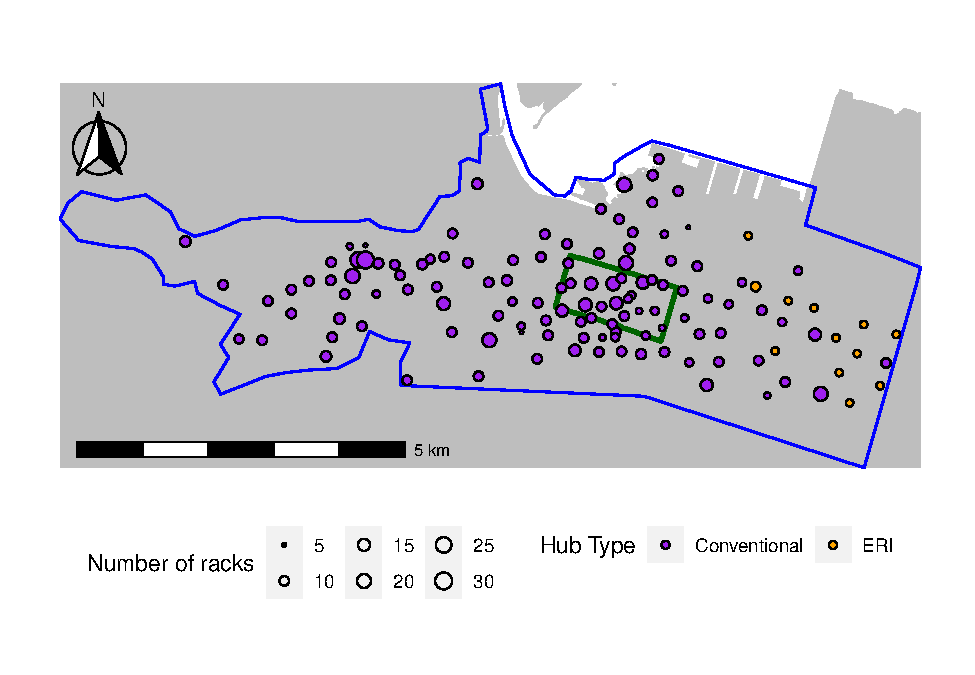
\includegraphics[width=1\linewidth]{Bike-share-spatial-equity-R1_files/figure-latex/sobi-stations-in-hamilton-1} 
%DIFDELCMD < %%%
\DIFdelendFL \DIFaddbeginFL 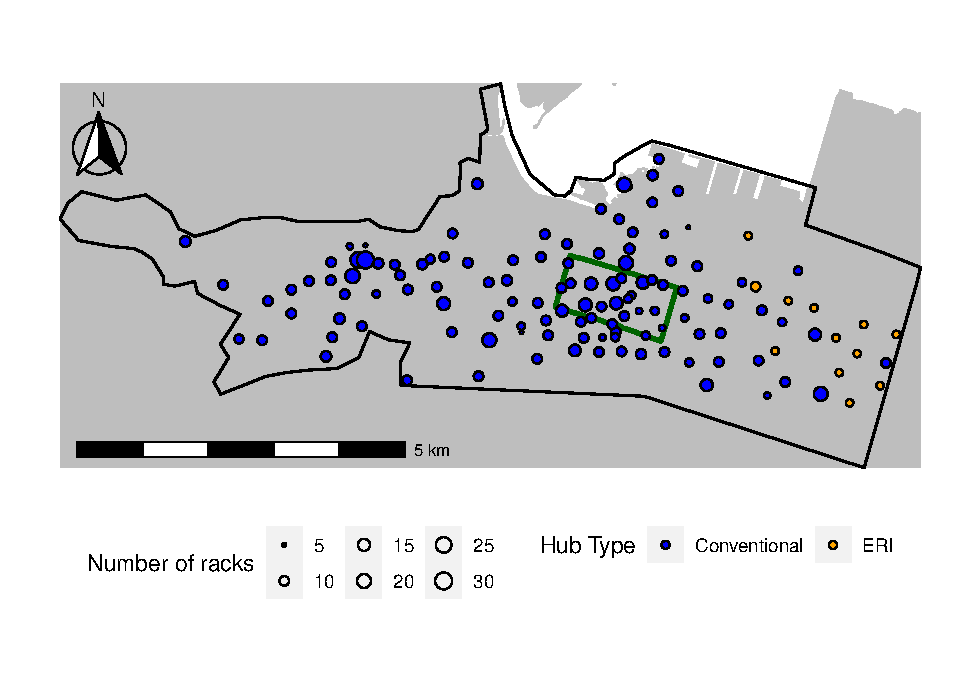
\includegraphics[width=1\linewidth]{Bike-share-spatial-equity_files/figure-latex/sobi-stations-in-hamilton-1} 
\DIFaddendFL 

}

\caption{The spatial distribution of bike share docking stations in Hamilton, Ontario. Conventional stations are in purple and equity (ERI) stations are in orange. The service area of Hamilton Bike Share is outlined in blue and the city's downtown core is outlined in dark green. Hamilton Census Metropolitan Area is shown in grey.}\label{fig:sobi-stations-in-hamilton}
\end{figure}

\hypertarget{sec:methods}{%
\section{4. Methods and Data}\label{sec:methods}}

\hypertarget{balanced-floating-catchment-area}{%
\subsection{4.1. Balanced Floating Catchment
Area}\label{balanced-floating-catchment-area}}

The BFCA method was developed to address issues with demand and supply
inflation that result from the overlapping catchment areas produced by
earlier FCA methods (Paez et al., 2019). \DIFdelbegin \DIFdel{Paez }\DIFdelend \DIFaddbegin \DIFadd{Páez }\DIFaddend et al. (2019) adjusted the
impedance weights so that both supply and demand are proportionally
allocated. The result is a FCA method that balances the population and
level of service by eliminating the over-counting of population and
level of service that leads to distortions in demand and supply.

The first step in the FCA method is to allocate the population to be
serviced by each docking station:

\begin{equation}
\label{eq:population-allocation}
P_j = {\sum_{i = 1}^{n} P_i{w_{ij}}}
\end{equation}

As seen in the equation above, the population allocated to station \(j\)
is the weighted sum of the population in the region; a spatial weight
\(w_{ij}\) represents the friction that the population at \(i\) faces
when reaching station \(j\), and is usually given by a distance-decay
function, so that each station is assumed to service only a segment of
the population within a limited geographical range. \DIFdelbegin %DIFDELCMD < 

%DIFDELCMD < %%%
\DIFdel{Next, }\DIFdelend \DIFaddbegin \DIFadd{The level of service
of station \(j\) in bicycle racks per person is }\DIFaddend the supply at each
station (i.e., the maximum number of bicycle racks) \DIFdelbegin \DIFdel{is divided by its estimated service }\DIFdelend \DIFaddbegin \DIFadd{divided by the
}\DIFaddend population within the established catchment area\DIFdelbegin \DIFdel{; this gives the level of service of station
\(j\) in bicycle racks per person}\DIFdelend : \begin{equation}
\label{eq:level-of-service}
L_j = \frac{S_j}{P_j} = \frac{S_j}{{\sum_{i = 1}^{n} P_i{w_{ij}}}}
\end{equation}

\DIFdelbegin \DIFdel{Finally}\DIFdelend \DIFaddbegin \DIFadd{In the second step}\DIFaddend , the accessibility of population \DIFdelbegin \DIFdel{cell }\DIFdelend \DIFaddbegin \DIFadd{unit }\DIFaddend \(i\) is
calculated as the weighted sum of the level of service of all stations
that can be reached from there according to the spatial weights:
\begin{equation}
\label{eq:FCA-accessibility}
A_i = {\sum_{j = 1}^{J} L\DIFdelbegin \DIFdel{_j{w_{ji}}}\DIFdelend \DIFaddbegin \DIFadd{_j{w_{ij}}}\DIFaddend } = {\sum_{j = 1}^{J} \DIFdelbegin \DIFdel{\frac{S_j{w_{ji}}}{\sum_{i = 1}^{n} P_i{w_{ij}}}}\DIFdelend \DIFaddbegin \DIFadd{\frac{S_j{w_{ij}}}{\sum_{i = 1}^{n} P_i{w_{ij}}}}\DIFaddend }
\end{equation}

The balanced approach of \DIFdelbegin \DIFdel{Paez et al}\DIFdelend \DIFaddbegin \DIFadd{Páez et al. }\DIFaddend (2019) replaces the spatial weights
with normalized versions as follows\DIFdelbegin \DIFdel{: }\DIFdelend \DIFaddbegin \DIFadd{. In the first step, the population
is weighted with: }\DIFaddend \begin{equation}
\label{eq:spatial-weights}
{w_{ij}^{i} = \DIFdelbegin \DIFdel{\frac{w_{ij}}{\sum_{j = 1}^{J} {w_{ji}}}}\DIFdelend \DIFaddbegin \DIFadd{\frac{w_{ij}}{\sum_{j = 1}^{J} {w_{ij}}}}\DIFaddend }
\end{equation}

\noindent and \DIFdelbegin \DIFdel{: }\DIFdelend \DIFaddbegin \DIFadd{in the second step, the level of service is weighted
using: }\DIFaddend \begin{equation}
\label{eq:spatial-weights-2}
{w_{ij}^{j} = \DIFdelbegin \DIFdel{\frac{w_{ij}}{\sum_{j = 1}^{J} {w_{ji}}}}\DIFdelend \DIFaddbegin \DIFadd{\frac{w_{ij}}{\sum_{i = 1}^{n} {w_{ij}}}}\DIFaddend }
\end{equation}

These weights satisfy the following properties: \begin{equation}
\label{eq:weights}
\sum_{j = 1}^{J} {w^i\DIFdelbegin \DIFdel{_{ji}}\DIFdelend \DIFaddbegin \DIFadd{_{ij}}\DIFaddend } = 1
\end{equation}

\noindent and: \begin{equation}
\label{eq:weights-2}
\sum_{i = 1}^{n} {w^j\DIFdelbegin \DIFdel{_{ji}}\DIFdelend \DIFaddbegin \DIFadd{_{ij}}\DIFaddend } = 1
\end{equation}

With these weights, accessibility can be calculated without risk of
demand or supply inflation: \begin{equation}
\label{eq:balanced-accessibility}
A_i = {\sum_{j = 1}^{J} \frac{S_j{w^j_{ij}}}{\sum_{i = 1}^{n} P_i{w^i_{ij}}}}
\end{equation}

By allocating the population and level of service proportionally, this
method preserves the values of the population and level of service
since: \begin{equation}
\label{eq:proportionality}
\sum_{i=1}^n A_i = \sum_{j=1}^J L_j
\end{equation}

In fact, since the proportional allocation procedure means that any
proportion of the population allocated to a station is never allocated
to other stations, and conversely any level of service allocated to a
population is never re-allocated elsewhere, this property is replicated
for any level of aggregation.

\hypertarget{pycnophylactic-interpolation}{%
\subsection{4.2. Pycnophylactic
Interpolation}\label{pycnophylactic-interpolation}}

Since walking trips to a docking station likely happen at a level lower
than even the smallest census geography, this requires a more
disaggregated approach than the use of census geographies. For this
reason, we implemented our analysis parting from \DIFdelbegin \DIFdel{micro population zones
}\DIFdelend \DIFaddbegin \DIFadd{small population cells
}\DIFaddend to better reflect the friction of walking to a docking station, which is
an important component of a bike share trip (Chen et al., 2019).

To obtain population at sub-census geography levels, we used
pycnophylactic interpolation (Tobler, 1979). We obtained population data
from the 2016 Census of Canada for dissemination areas (DA), which is
the smallest publicly available census geography in Canada. These zonal
values of the population were interpolated to smaller polygons that are
50-by-50 m in size. Pycnophylactic interpolation involves smoothing out
the population from each DA while preserving total volume\DIFdelbegin %DIFDELCMD < {[}%%%
\DIFdel{see Figure
\ref{fig:da-population}{]}}\DIFdelend . When
interpolating the population at this high level of resolution, it is
important to ensure that population numbers \DIFdelbegin \DIFdel{were }\DIFdelend \DIFaddbegin \DIFadd{are }\DIFaddend not allocated to areas
where people do not live in Hamilton (for example, to parks or large
institutional buildings, etc.). To do so, we retrieved shapefiles for
various geographic features from Open Hamilton. Next, we removed these
features from the PBSP core service area and used pycnophylactic
interpolation to disaggregate and reallocate population within the
remaining area {[}see Figure \ref{fig:interpolated-population}{]}.

\begin{figure}

{\centering \DIFdelbeginFL %DIFDELCMD < 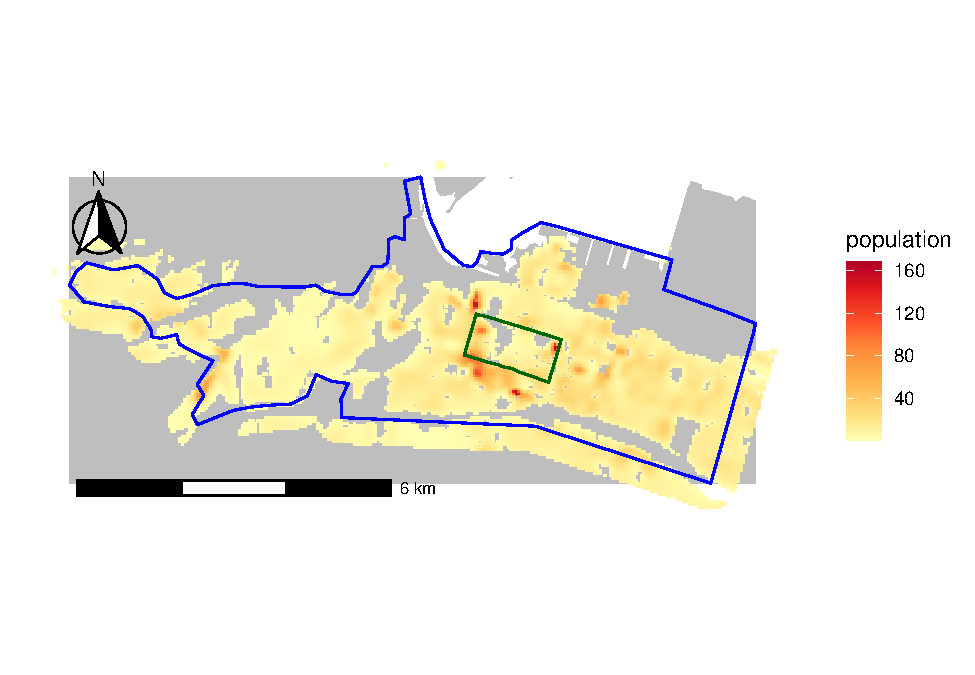
\includegraphics[width=0.9\linewidth]{Bike-share-spatial-equity-R1_files/figure-latex/interpolated-population-1} 
%DIFDELCMD < %%%
\DIFdelendFL \DIFaddbeginFL 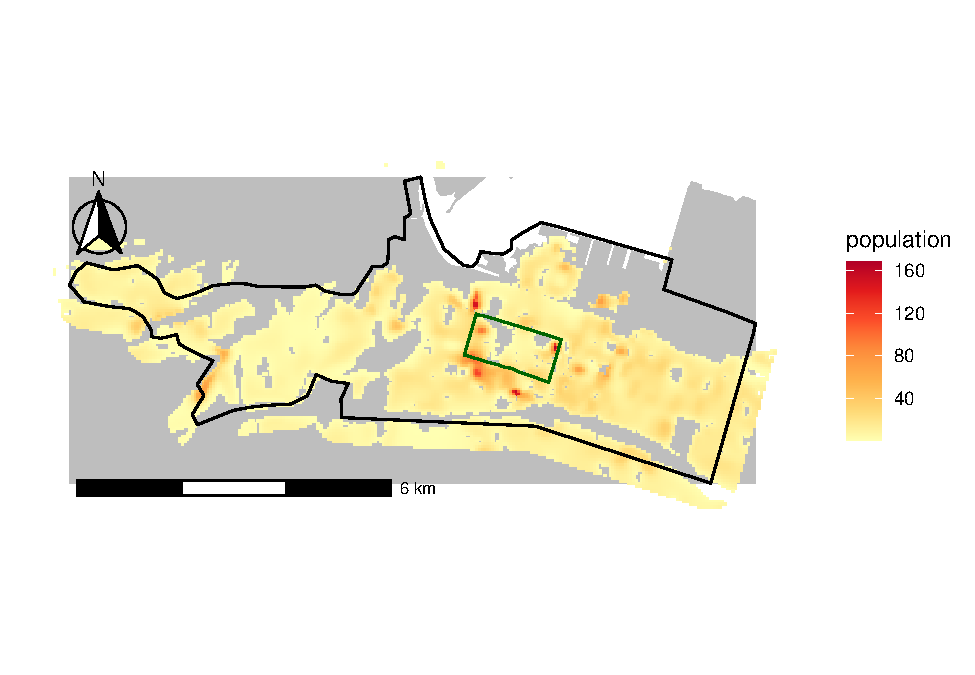
\includegraphics[width=0.9\linewidth]{Bike-share-spatial-equity_files/figure-latex/interpolated-population-1} 
\DIFaddendFL 

}

\caption{Interpolated population in Hamilton Bike Share's core service area (outlined in blue) and within 30 minutes of walking to the core service area. Each population cell is 50-by-50 m in size. The downtown area is outlined in dark green.}\label{fig:interpolated-population}
\end{figure}

\hypertarget{travel-time-matrix}{%
\subsection{4.3. Travel Time Matrix}\label{travel-time-matrix}}

To calculate walking times from the centroid of the \DIFdelbegin \DIFdel{micro }\DIFdelend population cells to
docking stations, we extracted OpenStreetMap data for HBS's service area
from \href{https://download.bbbike.org/osm/bbbike/}{BBBike}, an online
cycle route planner that interfaces with OpenStreetMap. OpenStreetMap
data provides the networks for calculating walking times from each
population cell to nearby docking stations, using a maximum walking
distance of 10 km and walking time of 30 minutes as thresholds. A travel
time matrix was created with the origins as the coordinates of the
population cells and the destinations as the coordinates of the docking
stations within the maximum threshold. This process provides a more
realistic measure of the friction of reaching stations by taking
infrastructure into account network travel times, rather than using the
Euclidean distance from population cell to station. Routing and travel
time calculations were completed using the \texttt{R} package
\texttt{r5r}, used for rapid realistic routing operations (Pereira et
al., 2021).

\hypertarget{data}{%
\subsection{4.4. Data}\label{data}}

All data for this research were accessed from publicly available Census
of Canada sources, from OpenStreetMaps, and from Open
Hamilton\footnote{https://open.hamilton.ca/}, a public online repository
of data curated by the City of Hamilton. Median total household income
statistics were drawn from the 2016 Canadian Census.

\hypertarget{results}{%
\section{5. Results}\label{results}}

\hypertarget{accessibility-by-distance-thresholds}{%
\subsection{5.1. Accessibility by Distance
Thresholds}\label{accessibility-by-distance-thresholds}}

Consensus regarding the distance that individuals are willing to walk to
access a docking station is lacking, but the literature on walking
behaviour provided some guidelines to determine the thresholds for our
sensitivity analysis. Previous studies have found that living within 250
m (Fuller et al., 2011) and 300 m (Kabra et al., 2020) of a docking
station is correlated with bike share use\DIFaddbegin \DIFadd{. Some studies have defined
``close proximity'' to a docking station as 500 metres or less (Fuller
et al., 2013; Hosford et al., 2019}\DIFaddend , \DIFaddbegin \DIFadd{2018), }\DIFaddend while other research has
found that walking trips are less than 600 m and rarely more than 1200 m
(Millward et al., 2013) or a median distance of 650 m (Larsen et al.,
2010). HBS will often depict a map at some docking stations to show the
locations of the other nearest stations within a five minute walk, which
suggests that this is an average distance that people are expected to
walk. The National Association of City Transportation Officials (NACTO)
has a similar normative guide (City Transportation Officials, 2015).

In the present case, we found that accessibility calculated using the
BFCA method increased with a threshold between two and four minutes, but
was then maximized at five minutes. Accessibility decreased
substantially after eight minutes, which is intuitive given that demand
on a limited supply increases as more people can reach each station.

We experimented with various thresholds by conducting a sensitivity
analysis to calculate accessibility at different walking times from
population cell to docking stations: three minutes, five minutes, ten
minutes, and fifteen minutes. We categorized these thresholds as
minimum, average, maximum, and extreme, respectively. At each threshold,
we compared accessibility between the current system and the original
system to examine the contribution of the twelve equity stations. When
considering the results reported below, it is important to remember that
accessibility is technically a form of smoothing (O'Kelly and Horner,
2003, pp. 7--8): smaller thresholds produce less smoothing (which can
result in ``spiky'' accessibility landscapes), while larger thresholds
produce more smoothing and fewer spikes.

\DIFaddbegin \DIFadd{In the analysis we use the following distance decay function: }\[
{\DIFadd{w_{ij} = \begin{cases} 
      1 & \text{when } t_{ij}\leq \gamma \\
      0 & \text{otherwise} 
   \end{cases}}}
\DIFadd{}\] \noindent \DIFadd{where \(\gamma\) is the relevant threshold. The weights are
standardized as discussed above.
}

\DIFaddend \hypertarget{minimum-threshold}{%
\subsubsection{5.1.1. Minimum Threshold}\label{minimum-threshold}}

With a walking distance of three minutes, we found that the total level
of service is 25.2 bicycle racks per person system-wide in the original
system configuration (i.e., without equity stations). The addition of
equity stations increases this slightly to 25.4 bicycles per person.
This total level of service is allocated to the population to obtain the
levels of accessibility, which turn out to be relatively uniform
overall, with the exception of two small areas where accessibility is
slightly higher. This high level of system-wide accessibility occurs
because the population that can reach a docking station when travel time
is three minutes or less is very limited, and accessibility is strongly
shaped by a few locations that concentrate population and stations. For
this reason, accessibility is highly concentrated in small areas around
those stations. The map is not shown, since it is less informative, but
can be recreated using the source code and data.

\hypertarget{average-threshold}{%
\subsubsection{5.1.2. Average Threshold}\label{average-threshold}}

With a walking distance of five minutes, we found that there are 68.6
bicycle racks per person system-wide in the original system
configuration (i.e., without equity stations). With the addition of
equity stations, there are now 68.8 bicycle racks per person. At this
threshold, there are more bicycle racks per person than at the minimum
threshold. System-wide accessibility has in fact increased: the
population that can reach the stations has grown, but not to the the
point that congestion effects begin to take place. Figure
\ref{fig:figure-7} presents a comparison of accessibility between the
systems. Again, accessibility is fairly uniform, with the exception of
one very small area. The equity stations noticeably increase
accessibility in the east end of the core service area by filling gaps
in PBSP coverage.

\begin{figure}

{\centering \DIFdelbeginFL %DIFDELCMD < \includegraphics[width=0.9\linewidth]{Bike-share-spatial-equity-R1_files/figure-latex/figure-7-1} 
%DIFDELCMD < %%%
\DIFdelendFL \DIFaddbeginFL \includegraphics[width=0.9\linewidth]{Bike-share-spatial-equity_files/figure-latex/figure-7-1} 
\DIFaddendFL 

}

\caption{Accessibility at 5 minutes walk (average threshold) compared between current system with equity stations and the original system without equity stations.}\label{fig:figure-7}
\end{figure}

\hypertarget{maximum-threshold}{%
\subsubsection{5.1.3. Maximum Threshold}\label{maximum-threshold}}

With a walking distance of ten minutes, we found that there are 3.61
bicycle racks per person system-wide in the original system
configuration (i.e., without equity stations). With the addition of
equity stations, there are now 3.74 bicycles per person. Figure
\ref{fig:figure-8} presents a comparison of accessibility between the
systems. Differences in accessibility across the service area are now
apparent, with users near the university and its adjacent neighborhoods,
as well as neighborhoods north of the downtown area (the latter is
outlined in green), having slightly higher accessibility. While the
differences are modest, they are more apparent at this threshold than at
shorter walking distances, especially in the more disadvantaged
neighbourhoods in the east end of the core service area where equity
stations were added.

\begin{figure}

{\centering \DIFdelbeginFL %DIFDELCMD < 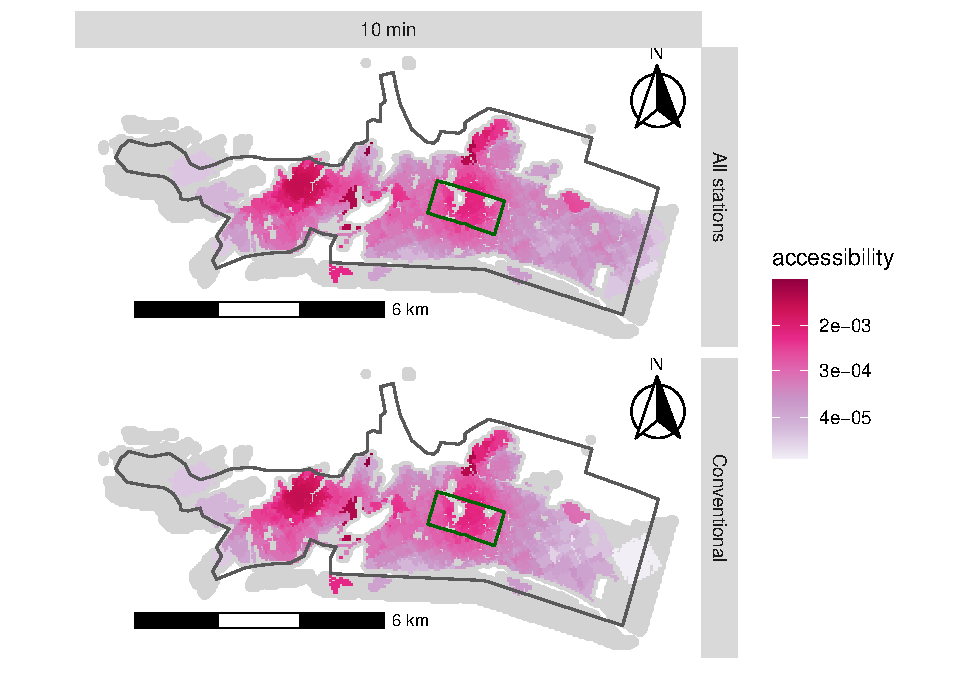
\includegraphics[width=0.9\linewidth]{Bike-share-spatial-equity-R1_files/figure-latex/figure-8-1} 
%DIFDELCMD < %%%
\DIFdelendFL \DIFaddbeginFL 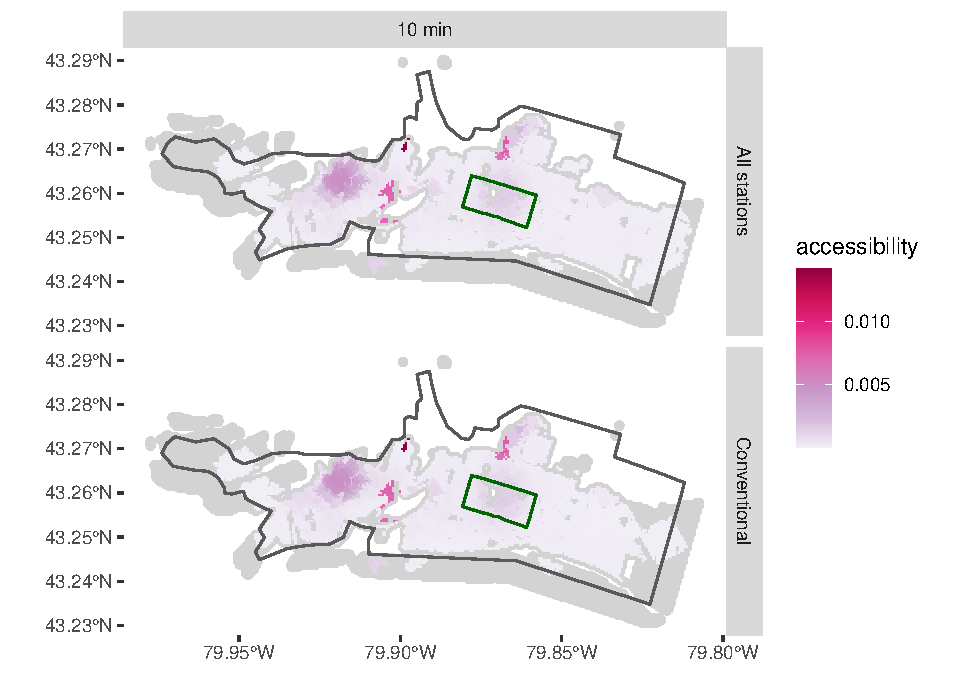
\includegraphics[width=0.9\linewidth]{Bike-share-spatial-equity_files/figure-latex/figure-8-1} 
\DIFaddendFL 

}

\caption{Accessibility at 10 minutes walk (maximum threshold) compared between current system with equity stations and the original system without equity stations.}\label{fig:figure-8}
\end{figure}

\hypertarget{extreme-threshold}{%
\subsubsection{5.1.4. Extreme Threshold}\label{extreme-threshold}}

With a walking distance of fifteen minutes, we found that there are 2.44
bicycle racks per person system-wide in the original system
configuration (i.e., without equity stations). With the addition of
equity stations, there are now 2.55 bicycles per person. Figure
\ref{fig:figure-9} presents a comparison of accessibility between the
systems. Users near the university and the neighborhoods north of the
downtown area (the latter is outlined in green) have the highest
accessibility, followed by those who live in the city's downtown area.
Accessibility in the east end, where equity stations were implemented,
of the core service area remains lower than other areas.

\begin{figure}

{\centering \DIFdelbeginFL %DIFDELCMD < \includegraphics[width=0.9\linewidth]{Bike-share-spatial-equity-R1_files/figure-latex/figure-9-1} 
%DIFDELCMD < %%%
\DIFdelendFL \DIFaddbeginFL \includegraphics[width=0.9\linewidth]{Bike-share-spatial-equity_files/figure-latex/figure-9-1} 
\DIFaddendFL 

}

\caption{Accessibility at 15 minutes walk (extreme threshold) compared between current system with equity stations and the original system without equity stations.}\label{fig:figure-9}
\end{figure}

\hypertarget{comparative-analysis}{%
\subsection{5.2. Comparative Analysis}\label{comparative-analysis}}

To highlight the benefit of using the BFCA approach, we conducted a
comparative analysis with the 2SFCA method. The latter method does not
allocate population and level of service proportionally, which means
that there are often substantial amounts of multiple counting each.
Figure \ref{fig:figure-10} shows the level of inflation and deflation at
five minutes that results when the balanced and the conventional FCA
methods are compared. The inflation and deflation is defined as the
ratio of the level of service and accessibility calculated using the
conventional approach to the balanced approach. This effect has been
documented in other studies (Chen et al., 2021; Paez et al., 2019).
Figure \ref{fig:figure-10} shows that in some locations the level of
service is deflated by up to 80\%. This is evident for the equity
stations in the east end of the core service area. Noticeably, the level
of service is least deflated in the downtown area, likely due to the
density of docking stations. Figure \ref{fig:figure-11} shows that
accessibility is inflated by as much as 50\% in many areas across the
city.

\begin{figure}

{\centering \DIFdelbeginFL %DIFDELCMD < 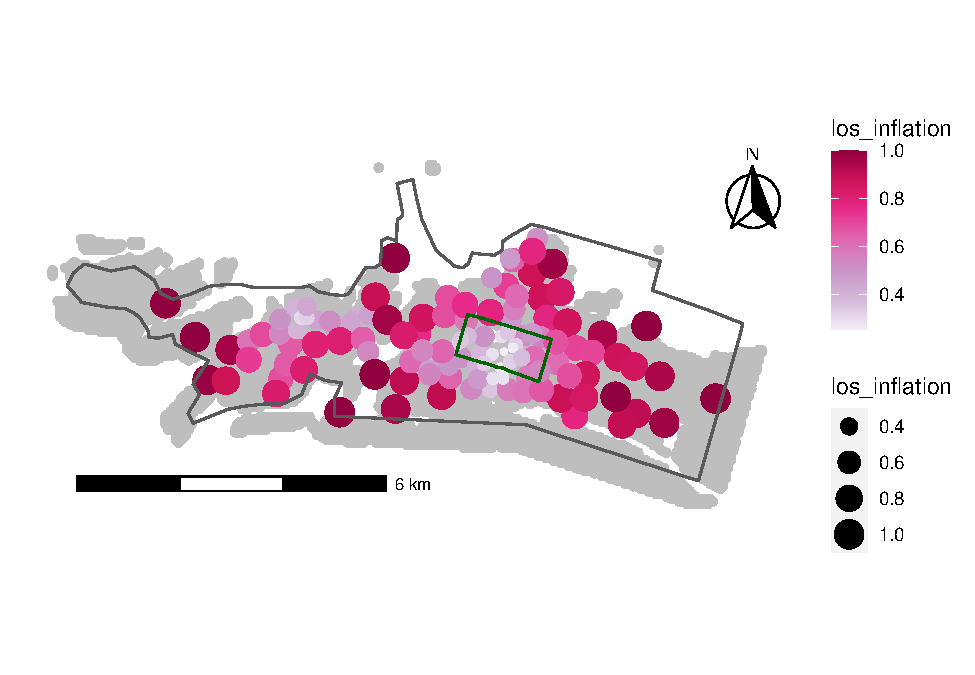
\includegraphics[width=0.9\linewidth]{Bike-share-spatial-equity-R1_files/figure-latex/figure-10-1} 
%DIFDELCMD < %%%
\DIFdelendFL \DIFaddbeginFL 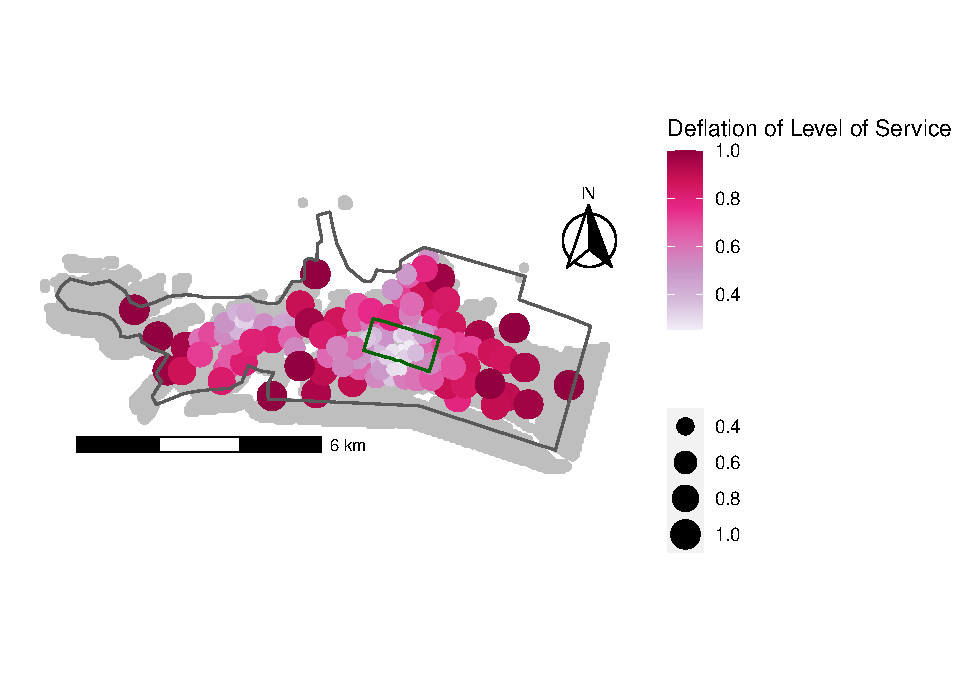
\includegraphics[width=0.9\linewidth]{Bike-share-spatial-equity_files/figure-latex/figure-10-1} 
\DIFaddendFL 

}

\caption{Deflation of level of service at 5 minutes walk (average threshold) in the current system with equity stations.}\label{fig:figure-10}
\end{figure}

\begin{figure}

{\centering \DIFdelbeginFL %DIFDELCMD < \includegraphics[width=0.9\linewidth]{Bike-share-spatial-equity-R1_files/figure-latex/figure-11-1} 
%DIFDELCMD < %%%
\DIFdelendFL \DIFaddbeginFL \includegraphics[width=0.9\linewidth]{Bike-share-spatial-equity_files/figure-latex/figure-11-1} 
\DIFaddendFL 

}

\caption{Inflation of accessibility at 5 minutes walk (average threshold) in the current system with equity stations.}\label{fig:figure-11}
\end{figure}

\hypertarget{accessibility-by-median-total-household-income}{%
\subsection{5.3. Accessibility by Median Total Household
Income}\label{accessibility-by-median-total-household-income}}

To examine whether accessibility to HBS was increased for groups with
lower income, we estimated what level of accessibility accrues to how
many people in different income strata. To this end, we took our \DIFdelbegin \DIFdel{micro
population zones }\DIFdelend \DIFaddbegin \DIFadd{small
population cells }\DIFaddend and aggregated the accessibility and population by the
median total household income as imputed from the dissemination areas. A
unique property of the BFCA method, which does not hold for the 2SFCA
approach because of the inflation/deflation issues discussed above, is
that accessibility and population data can be re-aggregated using income
as an aggregator criterion, while preserving the total population and
the level of service. This avoids demand and supply inflation, and also
enables us to present findings in a way that is more intuitive to
interpret. Figures \ref{fig:figure-bi-map-threshold-3},
\ref{fig:figure-bi-map-threshold-5},
\ref{fig:figure-bi-map-threshold-10}, and
\ref{fig:figure-bi-map-threshold-15} depict bivariate choropleth maps
that combine the spatial distribution of accessibility and median total
household income, using tertiles for the coloring scheme.

\begin{figure}
\DIFdelbeginFL %DIFDELCMD < 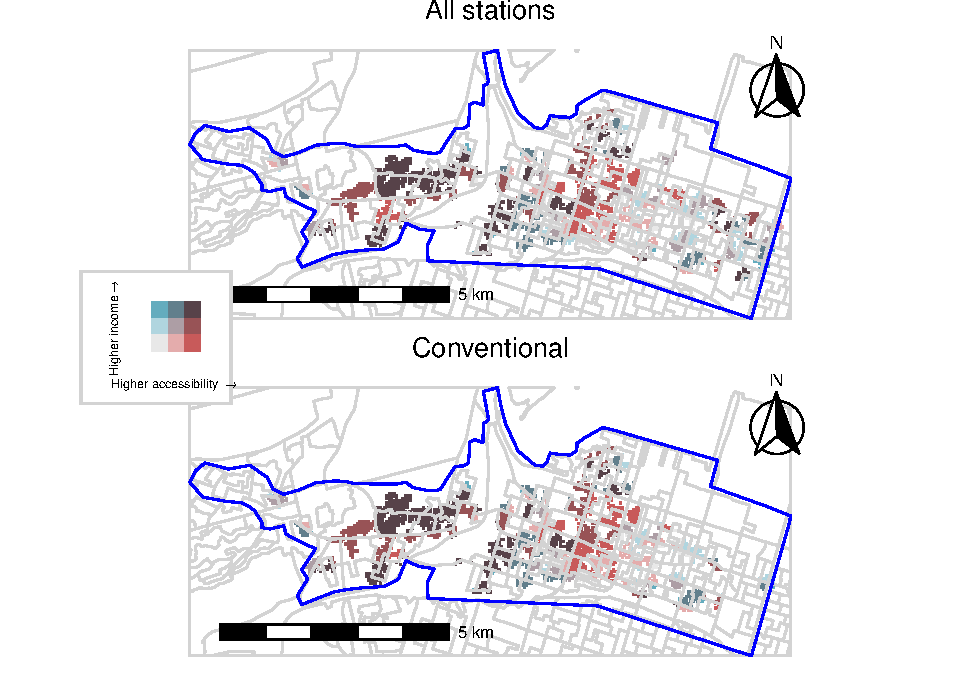
\includegraphics[width=1.2\linewidth]{Bike-share-spatial-equity-R1_files/figure-latex/figure-bi-map-threshold-3-1} %%%
\DIFdelendFL \DIFaddbeginFL 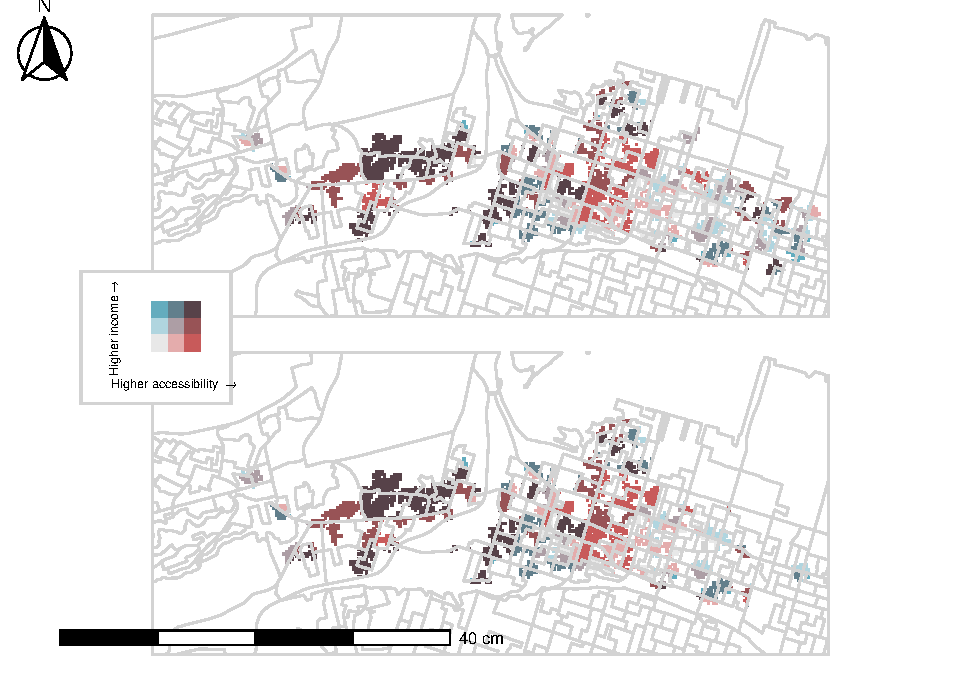
\includegraphics[width=1.2\linewidth]{Bike-share-spatial-equity_files/figure-latex/figure-bi-map-threshold-3-1} \DIFaddendFL \caption{\label{fig-bivariate-map-threshold-3}Bivariate map of accessibility and income at the minimum threshold of three minutes with equity stations (top panel) and without equity stations (bottom panel).}\label{fig:figure-bi-map-threshold-3}
\end{figure}

\begin{figure}
\DIFdelbeginFL %DIFDELCMD < 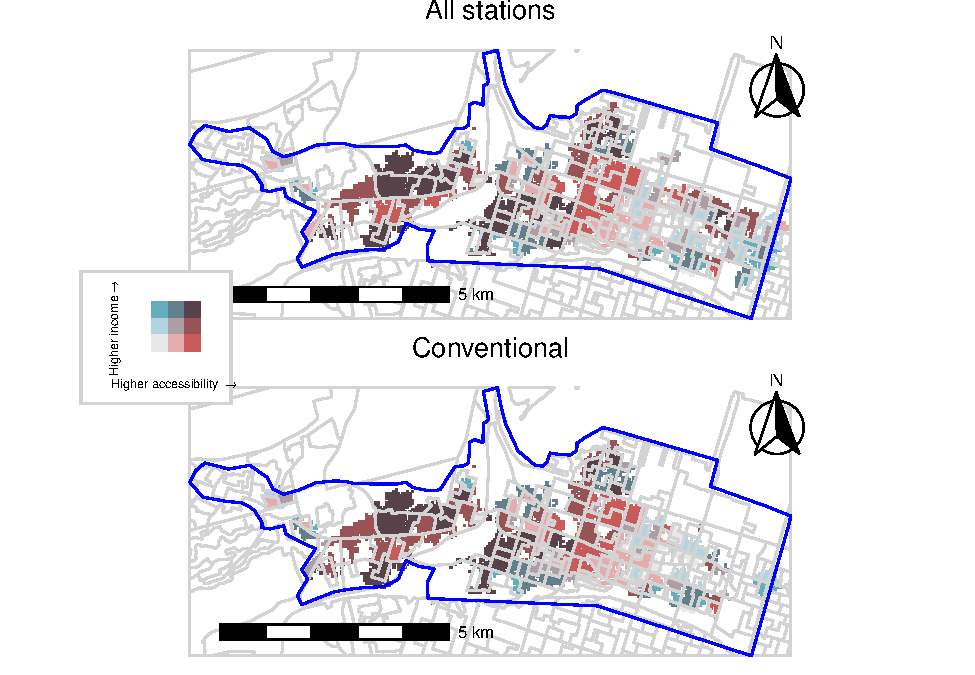
\includegraphics[width=1.2\linewidth]{Bike-share-spatial-equity-R1_files/figure-latex/figure-bi-map-threshold-5-1} %%%
\DIFdelendFL \DIFaddbeginFL 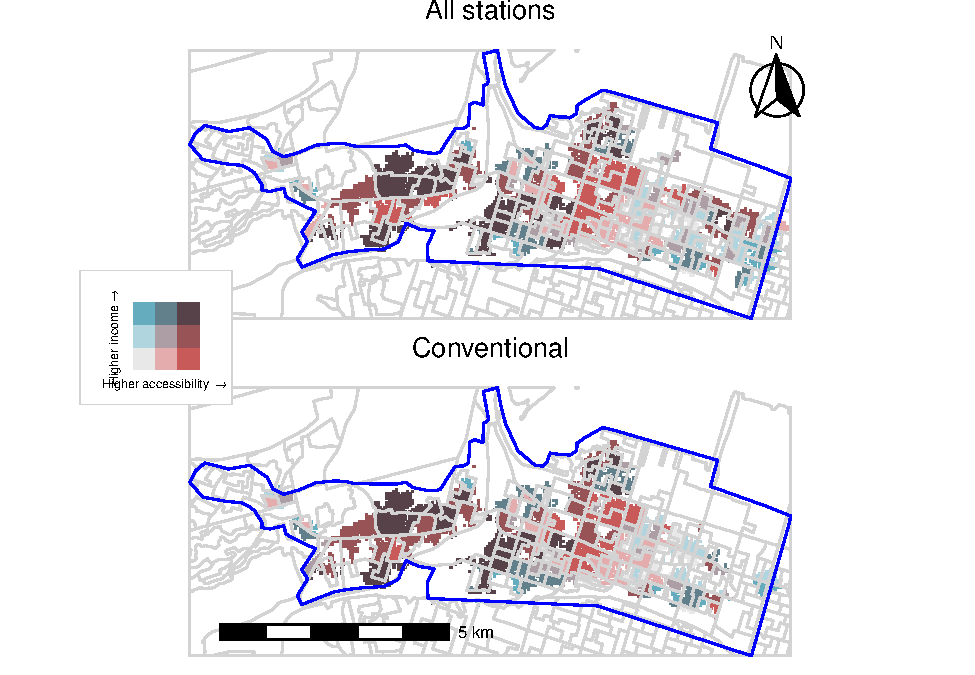
\includegraphics[width=1.2\linewidth]{Bike-share-spatial-equity_files/figure-latex/figure-bi-map-threshold-5-1} \DIFaddendFL \caption{\label{fig-bivariate-map-threshold-5}Bivariate map of accessibility and income at the average threshold of five minutes with equity stations (top panel) and without equity stations (bottom panel).}\label{fig:figure-bi-map-threshold-5}
\end{figure}

\begin{figure}
\DIFdelbeginFL %DIFDELCMD < 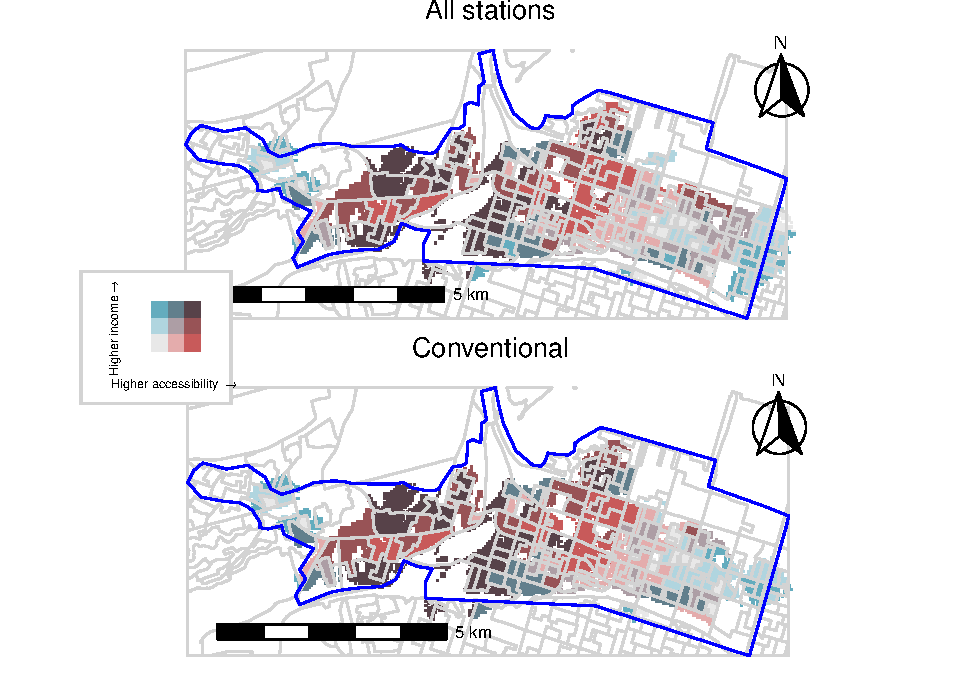
\includegraphics[width=1.2\linewidth]{Bike-share-spatial-equity-R1_files/figure-latex/figure-bi-map-threshold-10-1} %%%
\DIFdelendFL \DIFaddbeginFL 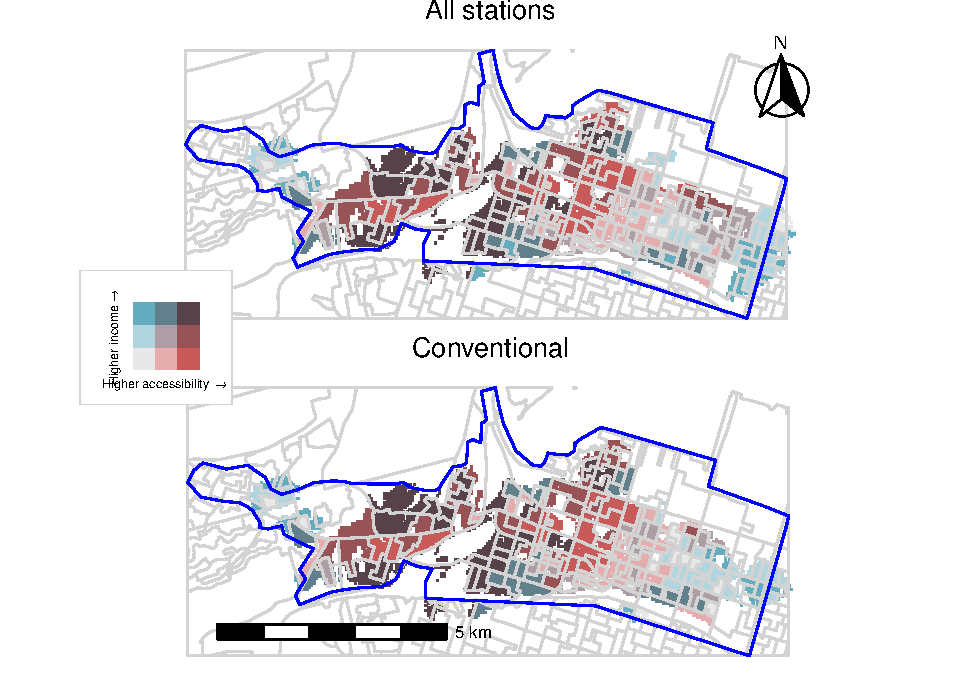
\includegraphics[width=1.2\linewidth]{Bike-share-spatial-equity_files/figure-latex/figure-bi-map-threshold-10-1} \DIFaddendFL \caption{\label{fig-bivariate-map-threshold-10}Bivariate map of accessibility and income at the maximum threshold of ten minutes with equity stations (top panel) and without equity stations (bottom panel).}\label{fig:figure-bi-map-threshold-10}
\end{figure}

\begin{figure}
\DIFdelbeginFL %DIFDELCMD < 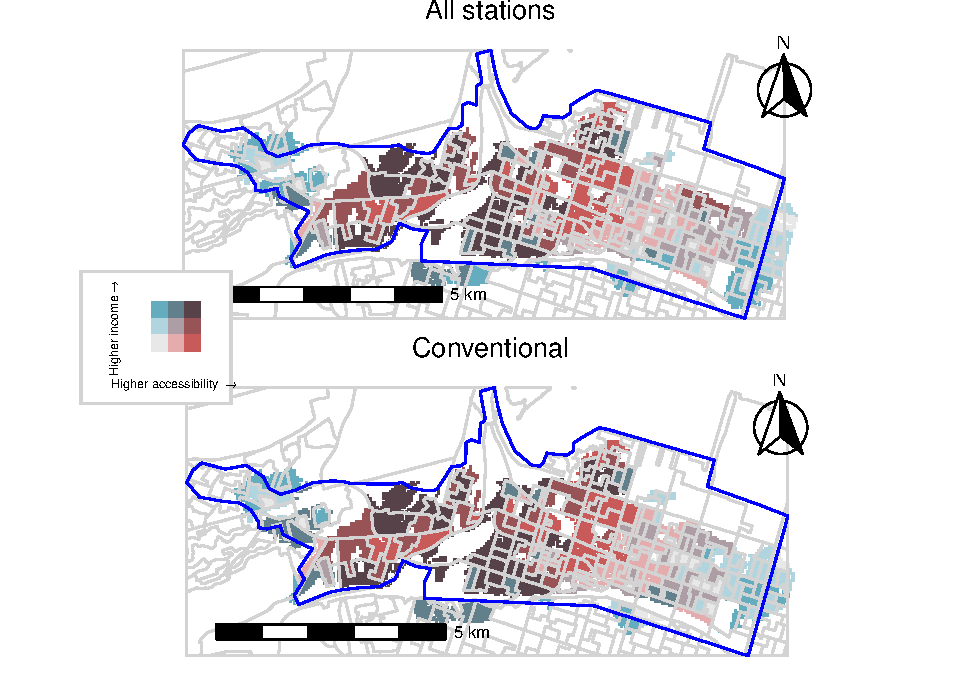
\includegraphics[width=1.2\linewidth]{Bike-share-spatial-equity-R1_files/figure-latex/figure-bi-map-threshold-15-1} %%%
\DIFdelendFL \DIFaddbeginFL 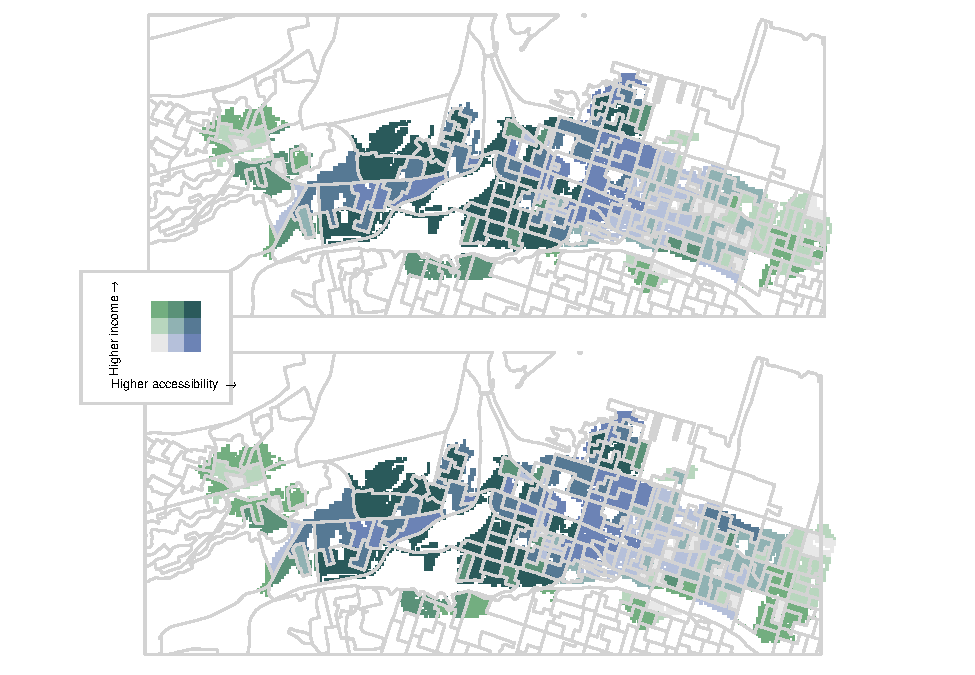
\includegraphics[width=1.2\linewidth]{Bike-share-spatial-equity_files/figure-latex/figure-bi-map-threshold-15-1} \DIFaddendFL \caption{\label{fig-bivariate-map-threshold-15}Bivariate map of accessibility and income at the extreme threshold of fifteen with equity stations (top panel) and without equity stations (bottom panel).}\label{fig:figure-bi-map-threshold-15}
\end{figure}

Table \ref{tab:accessibility-income} presents accessibility levels by
income strata. As expected, the extreme threshold of fifteen minutes is
associated with the largest number of people who are within the assumed
service area of docking stations. We found that stations added to HBS
expanded the spatial coverage of HBS, leading to more balance across the
core service area. This is particularly evident at the minimum and
average thresholds of three and five minutes, respectively, where the
equity stations fill a number of gaps in program coverage.

In line with Hosford and Winters' (2018) findings, we found that
accessibility to HBS was high for individuals in the bottom and second
quintiles of median total household income who live in the centre of the
core service area. This may well be an artifact of the spatial
socioeconomic and demographic profile of Hamilton, where the most dense
parts of the city (where a PBSP is most easily launched) are also those
with relatively lower incomes (Hosford and Winters, 2018). On the other
hand, we found the levels of accessibility to Hamilton's PBSP are
generally lower for populations in the bottom 20\% of median total
household income, compared to populations in the top 20\%.

Our analysis revealed that the addition of equity stations increased
accessibility to HBS by growing the population serviced irrespective of
the walking threshold. The largest gains were made for dissemination
areas in the second 20\% median total household income, where an
additional 3,073 and 5,395 people could reach a docking station within
three and five minutes walk, respectively, after the addition of equity
stations. However, we found that there were only small increases in the
population in the bottom 20\% of median total household income who are
serviced by the equity stations, and the accessibility gains are also
quite modest and smaller than for populations in the second and third
quintiles of median total household income. This suggests that
inequities in accessibility to HBS persist according to income, albeit
this depends on the walking time thresholds. With and without equity
stations, people in the top 20\% of income have the highest level of
access at a threshold of ten and fifteen minutes. Although dissemination
areas in the second 20\% have the highest level of access by a
significant amount at lower distance thresholds, the bottom 20\%, who
may benefit more from increased access to HBS, have the lowest
accessibility at three minutes threshold and the second lowest access at
all other thresholds.

\begin{table}

\caption{\label{tab:accessibility-income}\label{tab:accessibility-by-income}Accessibility and population serviced by income quintile and between systems (with and without equity stations). Total population is the population by income quintile in the DAs that have any PBSP service at all.}
\centering
\resizebox{\linewidth}{!}{
\begin{tabular}[t]{lccccccl}
\toprule
\multicolumn{2}{c}{ } & \multicolumn{2}{c}{Without Equity Stations} & \multicolumn{2}{c}{With Equity Stations} & \multicolumn{2}{c}{Difference} \\
\cmidrule(l{3pt}r{3pt}){3-4} \cmidrule(l{3pt}r{3pt}){5-6} \cmidrule(l{3pt}r{3pt}){7-8}
Income Quintile & Total Population & Population & Accessibility & Population & Accessibility & Population & Accessibility\\
\midrule
\addlinespace[0.3em]
\multicolumn{8}{l}{\textbf{Threshold - 3 minutes}}\\
\hspace{1em}\cellcolor{gray!6}{Bottom 20\%} & \cellcolor{gray!6}{43441} & \cellcolor{gray!6}{22359} & \cellcolor{gray!6}{2.377} & \cellcolor{gray!6}{22798} & \cellcolor{gray!6}{2.424} & \cellcolor{gray!6}{439} & \cellcolor{gray!6}{0.047}\\
\hspace{1em}Second 20\% & 33312 & 9347 & 12.203 & 12420 & 12.281 & 3073 & 0.078\\
\hspace{1em}\cellcolor{gray!6}{Third 20\%} & \cellcolor{gray!6}{30940} & \cellcolor{gray!6}{7745} & \cellcolor{gray!6}{3.093} & \cellcolor{gray!6}{9455} & \cellcolor{gray!6}{3.156} & \cellcolor{gray!6}{1710} & \cellcolor{gray!6}{0.063}\\
\hspace{1em}Fourth 20\% & 20185 & 1673 & 4.119 & 1673 & 4.119 & 0 & 0.000\\
\hspace{1em}\cellcolor{gray!6}{Top 20\%} & \cellcolor{gray!6}{27541} & \cellcolor{gray!6}{2151} & \cellcolor{gray!6}{3.757} & \cellcolor{gray!6}{2416} & \cellcolor{gray!6}{3.784} & \cellcolor{gray!6}{265} & \cellcolor{gray!6}{0.027}\\
\addlinespace[0.3em]
\multicolumn{8}{l}{\textbf{Threshold - 5 minutes}}\\
\hspace{1em}Bottom 20\% & 43441 & 35477 & 1.302 & 35803 & 1.357 & 326 & 0.055\\
\hspace{1em}\cellcolor{gray!6}{Second 20\%} & \cellcolor{gray!6}{33312} & \cellcolor{gray!6}{17513} & \cellcolor{gray!6}{56.048} & \cellcolor{gray!6}{22908} & \cellcolor{gray!6}{56.137} & \cellcolor{gray!6}{5395} & \cellcolor{gray!6}{0.089}\\
\hspace{1em}Third 20\% & 30940 & 15117 & 4.259 & 18309 & 4.291 & 3192 & 0.032\\
\hspace{1em}\cellcolor{gray!6}{Fourth 20\%} & \cellcolor{gray!6}{20185} & \cellcolor{gray!6}{2867} & \cellcolor{gray!6}{1.094} & \cellcolor{gray!6}{3116} & \cellcolor{gray!6}{1.095} & \cellcolor{gray!6}{249} & \cellcolor{gray!6}{0.001}\\
\hspace{1em}Top 20\% & 27541 & 4074 & 6.256 & 4540 & 6.264 & 466 & 0.008\\
\addlinespace[0.3em]
\multicolumn{8}{l}{\textbf{Threshold - 10 minutes}}\\
\hspace{1em}\cellcolor{gray!6}{Bottom 20\%} & \cellcolor{gray!6}{43441} & \cellcolor{gray!6}{41824} & \cellcolor{gray!6}{0.604} & \cellcolor{gray!6}{41981} & \cellcolor{gray!6}{0.622} & \cellcolor{gray!6}{157} & \cellcolor{gray!6}{0.018}\\
\hspace{1em}Second 20\% & 33312 & 27546 & 0.862 & 30503 & 0.929 & 2957 & 0.067\\
\hspace{1em}\cellcolor{gray!6}{Third 20\%} & \cellcolor{gray!6}{30940} & \cellcolor{gray!6}{22394} & \cellcolor{gray!6}{0.776} & \cellcolor{gray!6}{25128} & \cellcolor{gray!6}{0.802} & \cellcolor{gray!6}{2734} & \cellcolor{gray!6}{0.026}\\
\hspace{1em}Fourth 20\% & 20185 & 4544 & 0.225 & 4989 & 0.227 & 445 & 0.002\\
\hspace{1em}\cellcolor{gray!6}{Top 20\%} & \cellcolor{gray!6}{27541} & \cellcolor{gray!6}{7989} & \cellcolor{gray!6}{1.346} & \cellcolor{gray!6}{9078} & \cellcolor{gray!6}{1.348} & \cellcolor{gray!6}{1089} & \cellcolor{gray!6}{0.002}\\
\addlinespace[0.3em]
\multicolumn{8}{l}{\textbf{Threshold - 15 minutes}}\\
\hspace{1em}Bottom 20\% & 43441 & 42208 & 0.536 & 42327 & 0.557 & 119 & 0.021\\
\hspace{1em}\cellcolor{gray!6}{Second 20\%} & \cellcolor{gray!6}{33312} & \cellcolor{gray!6}{30507} & \cellcolor{gray!6}{0.555} & \cellcolor{gray!6}{31069} & \cellcolor{gray!6}{0.614} & \cellcolor{gray!6}{562} & \cellcolor{gray!6}{0.059}\\
\hspace{1em}Third 20\% & 30940 & 26108 & 0.554 & 26660 & 0.581 & 552 & 0.027\\
\hspace{1em}\cellcolor{gray!6}{Fourth 20\%} & \cellcolor{gray!6}{20185} & \cellcolor{gray!6}{6312} & \cellcolor{gray!6}{0.093} & \cellcolor{gray!6}{7435} & \cellcolor{gray!6}{0.096} & \cellcolor{gray!6}{1123} & \cellcolor{gray!6}{0.003}\\
\hspace{1em}Top 20\% & 27541 & 10209 & 0.808 & 11089 & 0.811 & 880 & 0.003\\
\bottomrule
\multicolumn{8}{l}{\rule{0pt}{1em}\textit{Note: }}\\
\multicolumn{8}{l}{\rule{0pt}{1em} }\\
\multicolumn{8}{l}{\rule{0pt}{1em}\textsuperscript{a} With equity stations = Hamilton Bike Share current system (118 conventional stations, 12 equity stations)}\\
\multicolumn{8}{l}{\rule{0pt}{1em}\textsuperscript{b} Without equity stations = Hamilton Bike Share original system (118 conventional stations, no equity stations)}\\
\end{tabular}}
\end{table}

\hypertarget{discussion}{%
\section{6. Discussion}\label{discussion}}

Using disaggregated population data, we examined equity in accessibility
to Hamilton Bike Share \DIFaddbegin \DIFadd{(HBS)}\DIFaddend , with a \DIFdelbegin \DIFdel{particular }\DIFdelend focus on assessing the contribution
of the program's equity stations. The BFCA approach, combined with
pycnophylactic interpolation, enabled us to measure accessibility on a
micro scale which better reflects the scale at which walking takes place
and avoids the ``absorption of disparities,'' as articulated by Chen et
al. (2019) and elsewhere in the transportation literature (National
Academies of Sciences, 2004; Rowangould et al., 2016). Our method also
considers \DIFaddbegin \DIFadd{potential }\DIFaddend demand and supply\DIFaddbegin \DIFadd{, as well as congestion effects, }\DIFaddend in
the calculation of accessibility, which is important for services like
PBSPs but not accounted for in other common accessibility models. Unlike
the 2SFCA method, there was no inflation or deflation in our
accessibility estimates because population and level of service were
preserved (see Figure \ref{fig:figure-10} and Figure
\ref{fig:figure-11}). This differentiates our analysis from similar
papers exploring equity in PBSPs that use larger geographical units of
analysis or that focus \DIFaddbegin \DIFadd{only }\DIFaddend on station location instead of level of
service. In this way, our paper has made an important contribution by
applying an intuitive and useful approach \DIFaddbegin \DIFadd{not previously used in the
cycling literature }\DIFaddend to measure accessibility to a PBSP. This open and
reproducible research could be expanded for additional analysis using
other individual-level data in Hamilton (e.g., age, gender, household
size, education, etc.) or applied to PBSPs in other North American
cities.

The sensitivity analysis revealed that accessibility to docking stations
is maximized at five minutes and decreases significantly by eight
minutes {[}see Table \ref{tab:accessibility-income}{]}. This reflects
the normative guide advertised on some docking stations in Hamilton
showing other stations within a five minute walk, as well as the
directive of NACTO (City Transportation Officials, 2015). We \DIFdelbegin \DIFdel{find }\DIFdelend \DIFaddbegin \DIFadd{found }\DIFaddend that
over 118,000 people can access a bike share station within a 15 minute
walk, which represents roughly 85\% of the total population in the core
service area {[}see Table \ref{tab:accessibility-income}{]}. At a
minimum threshold of three minutes, too few people can reach stations
which leads to relatively high levels of service since there is little
crowding for the stations. However, accessibility is at its lowest after
eight minutes whereby congestion effects due to increased potential
demand kick in. Chen et al. (2019) also found that accessibility
decreases as larger geographical units are used in the estimation, since
more people can access the service.

The City of Hamilton has recognized from the launch of HBS that
substantially more stations and bicycles are needed to service the area
(Hamilton, 2015a). With a service area of 40 sq.km, it is estimated that
Hamilton should have between 380 and 440 stations instead of 130, and
1,500 bicycles instead of 900 (Hamilton, 2015a). \DIFdelbegin \DIFdel{Reduced }\DIFdelend \DIFaddbegin \DIFadd{The City acknowledged
that reduced }\DIFaddend capacity within the system led to gaps in coverage in some
areas of the city ``with some areas not having the recommended station
density of 300m between stations or 10 stations per square km''
(Hamilton, 2015a). Figures \ref{fig:figure-bi-map-threshold-3},
\ref{fig:figure-bi-map-threshold-5},
\ref{fig:figure-bi-map-threshold-10}, and
\ref{fig:figure-bi-map-threshold-15} demonstrate how gaps in
\DIFdelbegin \DIFdel{service
}\DIFdelend \DIFaddbegin \DIFadd{accessibility }\DIFaddend were filled by the additional equity stations \DIFaddbegin \DIFadd{implemented
by Hamilton Bike Share}\DIFaddend . The improvement in accessibility is most
noticeable at the average and maximum thresholds in the east end of the
core service area, which corresponds to the neighbourhoods where
stations were added. However, the contribution of equity stations to
reducing inequities in accessibility was modest.

The equity stations were added to HBS as a targeted initiative to
increase access for \DIFdelbegin \DIFdel{disadvantaged communities}\DIFdelend \DIFaddbegin \DIFadd{equity users in specific under-serviced
neighbourhoods}\DIFaddend . However, we found that inequities persisted as evidenced
by differences in accessibility according to income quintile (Table
\ref{tab:accessibility-income}). While the addition of equity stations
seems to modestly increase accessibility for all income groups at all
thresholds, they did not increase accessibility substantially for any
single income group. Most importantly, individuals in the bottom 20\% of
median total household income have the second lowest level of access to
\DIFdelbegin \DIFdel{Hamilton Bike Share }\DIFdelend \DIFaddbegin \DIFadd{HBS }\DIFaddend at most thresholds (average, maximum, and extreme). At the minimum
threshold, the bottom 20\% have the lowest level of access. This
suggests that \DIFdelbegin \DIFdel{the equity stations may not have sufficiently
addressed
}\DIFdelend \DIFaddbegin \DIFadd{additional equity stations are needed to more sufficiently
address }\DIFaddend vertical equity. While previous research found that
neighborhoods with more disadvantage are better serviced by HBS, the
authors used the Pampalon Deprivation Index to determine the level of
disadvantage for dissemination areas \emph{across} the city not just
within the core service area (Hosford and Winters, 2018). Instead, we
used median total household income for each dissemination area
\emph{within} the core service area. We conclude that Hamilton's PBSP,
while by default located in areas with more deprivation compared to
other cities \DIFaddbegin \DIFadd{as noted by Hosford and Winters (2018)}\DIFaddend , continues to have
disparities in accessibility between income groups. With equity
stations, many areas with low median total household income in the east
end of the service area \DIFdelbegin \DIFdel{continue to }\DIFdelend have zero or low accessibility at the average
threshold of five minutes. At the maximum and extreme thresholds, the
top 20\% have the highest level of access to \DIFdelbegin \DIFdel{Hamilton
Bike Share}\DIFdelend \DIFaddbegin \DIFadd{HBS}\DIFaddend . These findings align
\DIFaddbegin \DIFadd{broadly }\DIFaddend with other studies from Tampa (Chen et al., 2019), Philadelphia
(Caspi and Noland, 2019) and Seattle (Mooney et al., 2019), which have
found disparities in station location, annual trips, or access to
bicycles, respectively, between levels of income and education. With the
addition of equity stations, there were large gains in accessibility for
the second 20\% at the average threshold, amounting to over 5,000 more
people, but much smaller gains for the bottom 20\% with only 326 more
people who are able to access a HBS station.

This paper highlights the importance of both the location and size of
docking stations for increasing equity in accessibility to PBSPs.
\DIFaddbegin \DIFadd{Congestion effects for services like bike share that offer a potential
maximum supply of bicycles (i.e., number of racks) at each docking
station must be taken into account when measuring accessibility. }\DIFaddend Several
studies have examined who can access PBSPs based on the location of
stations (among others, see Babagoli et al., 2019; Qian \DIFaddbegin \DIFadd{et al., 2020;
Qian }\DIFaddend and Jaller, 2020; Wang and Lindsey, 2019b\DIFdelbegin \DIFdel{;
}\textbf{\DIFdel{qianEnhancingEquitableService2020?}}%DIFAUXCMD
\DIFdelend ), but the size of docking
stations in disadvantaged communities is not considered in the
literature. \DIFdelbegin \DIFdel{Station size (i.e., potential maximum supply of bicycles)}\DIFdelend \DIFaddbegin \DIFadd{An exception is a study on bike share ridership in New York
City that found ``the number of docks at a bike share station is
statistically significant and positively associated with trip
attractions for both men and women'' (Wang and Akar, 2019, p. 5).
Station size }\DIFaddend was also not identified by PBSP owners and operators as a
factor that needed to be addressed in equity efforts (Howland et al.,
2017). PBSPs may not necessarily reduce inequities in access if stations
are easy to reach for \DIFdelbegin \DIFdel{disadvantaged groups }\DIFdelend \DIFaddbegin \DIFadd{equity users }\DIFaddend but offer only a small number of
bicycles. Likewise, more people may not opt to use the program if the
supply of bicycles available at nearby stations is insufficient to meet
demand. Babgoli et al. (2019) found a slight but not statistically
significant increase in the proportion of neighborhoods with the highest
levels of poverty that had stations after the Citi Bike expansion in
2015. Although the Citi Bike expansion was not specifically driven by a
desire to reduce inequity in access, 16\% of neighborhoods with the
highest levels of poverty had stations compared to 12\% before. This
leaves open the question as to whether the stations held enough bicycles
to meet demand, and whether congestion effects in neighbourhoods with
more poverty are reducing the potential of bike share trips.

The following policy and planning implications can inform efforts for
increasing equity in \DIFdelbegin \DIFdel{Hamilton Bike Share}\DIFdelend \DIFaddbegin \DIFadd{HBS}\DIFaddend , and potentially other PBSPs in North America.
Our analysis has identified specific areas that have both low
accessibility and low median total household income. Figures
\ref{fig:figure-bi-map-threshold-3},
\ref{fig:figure-bi-map-threshold-5},
\ref{fig:figure-bi-map-threshold-10}, and
\ref{fig:figure-bi-map-threshold-15} highlight potential locations for
new equity stations to \DIFdelbegin \DIFdel{better accommodate low income }\DIFdelend \DIFaddbegin \DIFadd{increase access for low-income }\DIFaddend groups. Additional
stations are needed to further reduce inequities in accessibility. This
information will be useful to transportation planners in Hamilton and
HBS operators. Our findings also suggest that PBSPs should consider
increasing the size of stations in \DIFdelbegin \DIFdel{disadvantaged communities. }\DIFdelend \DIFaddbegin \DIFadd{targeted communities. Notably, figure
\ref{fig:sobi-stations-in-hamilton} highlights how the equity stations
in Hamilton have a lower number of racks compared to docking stations in
the city's downtown core. }\DIFaddend Docking stations added to \DIFdelbegin \DIFdel{target }\DIFdelend \DIFaddbegin \DIFadd{increase }\DIFaddend vertical
equity should have an adequate supply of public bicycles, particularly
more in areas that have a strong interest in adopting bike share\DIFaddbegin \DIFadd{, to
increase levels of service and potentially attract new users}\DIFaddend . Finally,
distance to stations is associated with bike share use (Fuller et al.,
2011; Wang and Lindsey, 2019b), especially when the trip starts at the
residence (Fishman et al., 2013). Distance can also be a barrier to
using PBSPs (Fishman et al., 2014). To address this issue,
transportation planners and PBSP operators should consult with groups
and communities who are under-represented among bike share users to
determine how far they are willing to walk to reach a docking station
and to get their input on the location of new docking stations.

\hypertarget{study-limitations}{%
\section{7. Study Limitations}\label{study-limitations}}

This paper did not examine or compare ridership data between
conventional and equity stations. Therefore, further research is needed
to determine whether the addition of equity stations encouraged more
bicycling for \DIFdelbegin \DIFdel{disadvantaged groups }\DIFdelend \DIFaddbegin \DIFadd{equity users }\DIFaddend living near them. Other studies have
specifically looked at differences in trip type, frequency, or length
among users from disadvantaged neighborhoods (Caspi and Noland, 2019;
Qian and Jaller, 2020; Wang and Lindsey, 2019a), but our analysis is
limited by the lack of publicly available route and individual user data
to conduct similar analyses for HBS.

An additional limitation is the lack of publicly available information
about the average number of bicycles at each station on a daily basis.
HBS works to balance the number of bicycles across the core service
area, but it is reasonable to expect that the number of bicycles will
not match exactly the number of racks at every station. Ideally, instead
of number of bicycle racks as our measure of supply, we would have liked
to use the average number of bicycles at stations, perhaps at different
times during the day across many seasons. Should this data become
available, it would be worthwhile to revisit the \DIFdelbegin \DIFdel{question }\DIFdelend \DIFaddbegin \DIFadd{study }\DIFaddend to examine how
well the operation of the system (including balancing of bicycles across
stations) works to maintain the nominal levels of accessibility examined
in this paper.

\hypertarget{conclusion}{%
\section{8. Conclusion}\label{conclusion}}

The addition of specific stations to improve equity within the PBSP in
Hamilton had the net effect of increasing accessibility and reducing
vertical inequities to some extent. In particular, accessibility
improved the most for those in the second 20\% median total household
income at all thresholds, but the gains were only modest for all income
groups. Dissemination areas in the bottom 20\% had the lowest
accessibility at three minutes, and second lowest levels of
accessibility at five, ten, and fifteen minutes. Congestion effects were
observed at higher thresholds, with accessibility decreasing
significantly once the catchment area is increased to ten minutes
walking.

Wang and Lindsey (2019b) have noted that there is a lack of research
that examines how bike share users' behaviour changes as a result of
program changes to station locations or improvements in accessibility.
As such, a logical next step to this research is to examine whether the
equity stations increased ridership or resulted in new memberships \DIFdelbegin \DIFdel{in
areas that were previously under-serviced}\DIFdelend \DIFaddbegin \DIFadd{for
equity users}\DIFaddend . An examination of the types of trips undertaken by
residents in these areas would also be informative, such as the study
undertaken by Caspi and Norland (2019) after \DIFdelbegin \DIFdel{bike share }\DIFdelend \DIFaddbegin \DIFadd{docking }\DIFaddend stations were
implemented in low-income Philadelphia neighborhoods. The bulk of
\DIFdelbegin \DIFdel{cycling facilities that have }\DIFdelend \DIFaddbegin \DIFadd{bicycle infrastructure that has }\DIFaddend been built in Hamilton to date \DIFdelbegin \DIFdel{are }\DIFdelend \DIFaddbegin \DIFadd{is
}\DIFaddend located in the core service area \DIFaddbegin \DIFadd{particularly }\DIFaddend near the conventional
stations. It would be worthwhile to explore the route choice of bike
share trips departing or ending at the equity stations and to identify
factors that specifically influence trips from these stations, which
would extend existing studies conducted by Scott and colleagues (Lu et
al., 2018; Scott et al., 2021; Scott and Ciuro, 2019). \DIFaddbegin \DIFadd{Perceived
accessibility using bike share according to low-income neighbourhoods
could also be studied in the future. Lättman et al. (2016) have
developed the }\emph{\DIFadd{Perceived Accessibility Scale}} \DIFadd{that would be useful
for this purpose. }\DIFaddend This paper, combined with additional studies such as
those conceptualized above, would serve as a valuable case study for
Hamilton and other cities with PBSPs that wish to evaluate and address
inequities in accessibility \DIFdelbegin \DIFdel{and }\DIFdelend \DIFaddbegin \DIFadd{to active }\DIFaddend transportation options in urban
areas.

\hypertarget{acknowledgments}{%
\section{Acknowledgments}\label{acknowledgments}}

We wish to thank the anonymous reviewers who provided constructive
feedback to improve the quality of our paper. This research was
completed using open software, and we also wish to acknowledge the
developers of the following \texttt{R} packages: \texttt{biscale}
(Prener et al., 2020), \texttt{cowplot} (Wilke, 2020),
\texttt{data.table} (Dowle and Srinivasan, 2021), \texttt{disk.frame}
(ZJ, 2021), \texttt{gdistance} (van Etten, 2020), \texttt{gridExtra}
(Auguie, 2017), \texttt{kableExtra} (Zhu, 2021), \texttt{knitr} (Xie,
2021a), \texttt{pycno} (Brunsdon, 2014), \texttt{r5r} (Saraiva et al.,
2021), \texttt{raster} (Hijmans, 2021), \texttt{rgdal} (Bivand et al.,
2021), \texttt{rticles} (Allaire et al., 2021), \texttt{sf} (Pebesma,
2021), \texttt{tidyverse} (Wickham, 2021), \texttt{tinytex} (Xie,
2021b), \texttt{units} (Pebesma et al., 2021).

\hypertarget{references}{%
\section*{References}\label{references}}
\addcontentsline{toc}{section}{References}

\hypertarget{refs}{}
\begin{CSLReferences}{1}{0}
\leavevmode\hypertarget{ref-R-rticles}{}%
Allaire, J., Xie, Y., R Foundation, Wickham, H., Journal of Statistical
Software, Vaidyanathan, R., Association for Computing Machinery,
Boettiger, C., Elsevier, Broman, K., Mueller, K., Quast, B., Pruim, R.,
Marwick, B., Wickham, C., Keyes, O., Yu, M., Emaasit, D., Onkelinx, T.,
Gasparini, A., Desautels, M.-A., Leutnant, D., MDPI, Taylor and Francis,
Ögreden, O., Hance, D., Nüst, D., Uvesten, P., Campitelli, E.,
Muschelli, J., Hayes, A., Kamvar, Z.N., Ross, N., Cannoodt, R., Luguern,
D., Kaplan, D.M., Kreutzer, S., Wang, S., Hesselberth, J., Dervieux, C.,
2021. Rticles: Article formats for r markdown.

\leavevmode\DIFaddbegin \hypertarget{ref-arribas2021open}{}%DIF > 
\DIFadd{Arribas/Bel, D., Green, M., Rowe, F., Singleton, A., 2021. Open data
products: A framework for creating valuable analysis-ready data. Journal
of Geographical Systems.
doi:}\href{https://doi.org/10.1007/s10109-021-00361-7}{\DIFadd{10.1007/s10109-021-00361-7}}

\leavevmode\DIFaddend \hypertarget{ref-auchinclossDesignBaselineDescription2020}{}%
Auchincloss, A.H., Michael, Y.L., Fuller, D., Li, S., Niamatullah, S.,
Fillmore, C.E., Setubal, C., Bettigole, C., 2020. Design and baseline
description of a cohort of bikeshare users in the city of
{Philadelphia}. Journal of Transport \& Health 16, 100836.
doi:\href{https://doi.org/10.1016/j.jth.2020.100836}{10.1016/j.jth.2020.100836}

\leavevmode\hypertarget{ref-R-gridExtra}{}%
Auguie, B., 2017. gridExtra: Miscellaneous functions for "grid"
graphics.

\leavevmode\hypertarget{ref-babagoliExploringHealthSpatial2019}{}%
Babagoli, M.A., Kaufman, T.K., Noyes, P., Sheffield, P.E., 2019.
Exploring the health and spatial equity implications of the {New York
City Bike} share system. Journal of Transport \& Health 13, 200--209.
doi:\href{https://doi.org/10.1016/j.jth.2019.04.003}{10.1016/j.jth.2019.04.003}

\leavevmode\hypertarget{ref-R-rgdal}{}%
Bivand, R., Keitt, T., Rowlingson, B., 2021. Rgdal: Bindings for the
geospatial data abstraction library.

\leavevmode\hypertarget{ref-bivand2020progress}{}%
Bivand, R.S., 2020. Progress in the r ecosystem for representing and
handling spatial data. Journal of Geographical Systems 1--32.
doi:\href{https://doi.org/10.1007/s10109-020-00336-0}{10.1007/s10109-020-00336-0}

\leavevmode\hypertarget{ref-breyWantRideMy2017}{}%
Brey, R., Castillo-Manzano, J.I., Castro-Nuño, M., 2017. 'I want to ride
my bicycle': Delimiting cyclist typologies. Applied Economics Letters
24, 549--552.
doi:\href{https://doi.org/10.1080/13504851.2016.1210760}{10.1080/13504851.2016.1210760}

\leavevmode\hypertarget{ref-R-pycno}{}%
Brunsdon, C., 2014. Pycno: Pycnophylactic interpolation.

\leavevmode\hypertarget{ref-brunsdon2020opening}{}%
Brunsdon, C., Comber, A., 2020. Opening practice: Supporting
reproducibility and critical spatial data science. Journal of
Geographical Systems 1--20.
doi:\href{https://doi.org/10.1007/s10109-020-00334-2}{10.1007/s10109-020-00334-2}

\leavevmode\hypertarget{ref-buckAreBikeshareUsers2013}{}%
Buck, D., Buehler, R., Happ, P., Rawls, B., Chung, P., Borecki, N.,
2013. Are bikeshare users different from regular cyclists?: A first look
at short-term users, annual members, and area cyclists in the
washington, d.c., region. Transportation Research Record 2387, 112--119.
doi:\href{https://doi.org/10.3141/2387-13}{10.3141/2387-13}

\leavevmode\hypertarget{ref-caspiBikesharingPhiladelphiaLowerincome2019}{}%
Caspi, O., Noland, R.B., 2019. Bikesharing in {Philadelphia}: {Do}
lower-income areas generate trips? Travel Behaviour and Society 16,
143--152.
doi:\href{https://doi.org/10.1016/j.tbs.2019.05.004}{10.1016/j.tbs.2019.05.004}

\leavevmode\hypertarget{ref-chenMeasuringAccessibilityHealth2021}{}%
Chen, W., Cheng, L., Chen, X., Chen, J., Cao, M., 2021. Measuring
accessibility to health care services for older bus passengers: {A}
finer spatial resolution. Journal of Transport Geography 93, 103068.
doi:\href{https://doi.org/10.1016/j.jtrangeo.2021.103068}{10.1016/j.jtrangeo.2021.103068}

\leavevmode\hypertarget{ref-chenExploringEquityPerformance2019}{}%
Chen, Z., Guo, Y., Stuart, A.L., Zhang, Y., Li, X., 2019. Exploring the
equity performance of bike-sharing systems with disaggregated data: {A}
story of southern {Tampa}. Transportation Research Part A: Policy and
Practice 130, 529--545.
doi:\href{https://doi.org/10.1016/j.tra.2019.09.048}{10.1016/j.tra.2019.09.048}

\leavevmode\hypertarget{ref-chenUnobservedHeterogeneityTransportation2021}{}%
Chen, Z., Li, X., 2021. Unobserved heterogeneity in transportation
equity analysis: {Evidence} from a bike-sharing system in southern
{Tampa}. Journal of Transport Geography 91, 102956.
doi:\href{https://doi.org/10.1016/j.jtrangeo.2021.102956}{10.1016/j.jtrangeo.2021.102956}

\leavevmode\hypertarget{ref-nactowalkingstation2015}{}%
City Transportation Officials, N.A. of, 2015. Walkable station spacing
is key to successful, equitable bike share {[}WWW Document{]}. URL
\url{https://nacto.org/wp-content/uploads/2015/09/NACTO_Walkable-Station-Spacing-Is-Key-For-Bike-Share_Sc.pdf}

\leavevmode\hypertarget{ref-delamaterSpatialAccessibilitySuboptimally2013}{}%
Delamater, P.L., 2013. Spatial accessibility in suboptimally configured
health care systems: {A} modified two-step floating catchment area
({M2SFCA}) metric. Health \& Place 24, 30--43.
doi:\href{https://doi.org/10.1016/j.healthplace.2013.07.012}{10.1016/j.healthplace.2013.07.012}

\leavevmode\hypertarget{ref-delboscUsingLorenzCurves2011}{}%
Delbosc, A., Currie, G., 2011. Using {Lorenz} curves to assess public
transport equity. Journal of Transport Geography, Special section on
{Alternative Travel} futures 19, 1252--1259.
doi:\href{https://doi.org/10.1016/j.jtrangeo.2011.02.008}{10.1016/j.jtrangeo.2011.02.008}

\leavevmode\hypertarget{ref-R-data.table}{}%
Dowle, M., Srinivasan, A., 2021. Data.table: Extension of `data.frame`.

\leavevmode\hypertarget{ref-fishmanBikeshareReviewRecent2016}{}%
Fishman, E., 2016. Bikeshare: {A Review} of {Recent Literature}.
Transport Reviews 36, 92--113.
doi:\href{https://doi.org/10.1080/01441647.2015.1033036}{10.1080/01441647.2015.1033036}

\leavevmode\hypertarget{ref-fishmanBikeShareSynthesis2013}{}%
Fishman, E., Washington, S., Haworth, N., 2013. Bike {Share}: {A
Synthesis} of the {Literature}. Transport Reviews 33, 148--165.
doi:\href{https://doi.org/10.1080/01441647.2013.775612}{10.1080/01441647.2013.775612}

\leavevmode\DIFaddbegin \hypertarget{ref-fishmanBikeshareImpactActive2015}{}%DIF > 
\DIFadd{Fishman, E., Washington, S., Haworth, N., 2015. Bikeshare's impact on
active travel: }{\DIFadd{Evidence}} \DIFadd{from the }{\DIFadd{United States}}\DIFadd{, }{\DIFadd{Great Britain}}\DIFadd{, and
}{\DIFadd{Australia}}\DIFadd{. Journal of Transport \& Health 2, 135--142.
doi:}\href{https://doi.org/10.1016/j.jth.2015.03.004}{\DIFadd{10.1016/j.jth.2015.03.004}}

\leavevmode\DIFaddend \hypertarget{ref-fishmanBarriersBikesharingAnalysis2014}{}%
Fishman, E., Washington, S., Haworth, N., Mazzei, A., 2014. Barriers to
bikesharing: An analysis from {Melbourne} and {Brisbane}. Journal of
Transport Geography 41, 325--337.
doi:\href{https://doi.org/10.1016/j.jtrangeo.2014.08.005}{10.1016/j.jtrangeo.2014.08.005}

\leavevmode\hypertarget{ref-fullerUseNewPublic2011}{}%
Fuller, D., Gauvin, L., Kestens, Y., Daniel, M., Fournier, M., Morency,
P., Drouin, L., 2011. Use of a {New Public Bicycle Share Program} in
{Montreal}, {Canada}. American Journal of Preventive Medicine 41,
80--83.
doi:\href{https://doi.org/10.1016/j.amepre.2011.03.002}{10.1016/j.amepre.2011.03.002}

\leavevmode\DIFaddbegin \hypertarget{ref-fullerImpactEvaluationPublic2013}{}%DIF > 
\DIFadd{Fuller, D., Gauvin, L., Kestens, Y., Daniel, M., Fournier, M., Morency,
P., Drouin, L., 2013. Impact evaluation of a public bicycle share
program on cycling: A case example of }{\DIFadd{BIXI}} \DIFadd{in }{\DIFadd{Montreal}}\DIFadd{, }{\DIFadd{Quebec}}\DIFadd{.
American Journal of Public Health 103, e85--92.
doi:}\href{https://doi.org/10.2105/AJPH.2012.300917}{\DIFadd{10.2105/AJPH.2012.300917}}

\leavevmode\hypertarget{ref-geursAccessibilityEvaluationLanduse2004}{}%DIF > 
\DIFadd{Geurs, K.T., van Wee, B., 2004. Accessibility evaluation of land-use and
transport strategies: Review and research directions. Journal of
Transport Geography 12, 127--140.
doi:}\href{https://doi.org/10.1016/j.jtrangeo.2003.10.005}{\DIFadd{10.1016/j.jtrangeo.2003.10.005}}

\leavevmode\DIFaddend \hypertarget{ref-hamiltonsobi2014}{}%
Hamilton, C. of, 2014. Hamilton bike share public engagement report
{[}WWW Document{]}. URL
\url{https://hamilton.socialbicycles.com/assets/pdf/Social_Cyclist_Bike_Share_Report.pdf}

\leavevmode\hypertarget{ref-hamiltonsobi2015}{}%
Hamilton, C. of, 2015a. Public bike share transit system implementation
plan (PW13015c) - (city wide) {[}WWW Document{]}. URL
\url{https://pub-hamilton.escribemeetings.com/filestream.ashx?DocumentId=118356}

\leavevmode\hypertarget{ref-hamiltonHamiltonBikeShare2015}{}%
Hamilton, C. of, 2015b. Hamilton {Bike Share}.

\leavevmode\hypertarget{ref-handyMeasuringAccessibilityExploration1997}{}%
Handy, S.L., Niemeier, D.A., 1997. Measuring {Accessibility}: {An
Exploration} of {Issues} and {Alternatives}. Environment and Planning A:
Economy and Space 29, 1175--1194.
doi:\href{https://doi.org/10.1068/a291175}{10.1068/a291175}

\leavevmode\hypertarget{ref-R-raster}{}%
Hijmans, R.J., 2021. Raster: Geographic data analysis and modeling.

\leavevmode\hypertarget{ref-hosfordEvaluationImpactPublic2018}{}%
Hosford, K., Fuller, D., Lear, S.A., Teschke, K., Gauvin, L., Brauer,
M., Winters, M., 2018. Evaluation of the impact of a public bicycle
share program on population bicycling in {Vancouver}, {BC}. Preventive
Medicine Reports 12, 176--181.
doi:\href{https://doi.org/10.1016/j.pmedr.2018.09.014}{10.1016/j.pmedr.2018.09.014}

\leavevmode\hypertarget{ref-hosfordWhoArePublic2018}{}%
Hosford, K., Winters, M., 2018. Who {Are Public Bicycle Share Programs
Serving}? {An Evaluation} of the {Equity} of {Spatial Access} to
{Bicycle Share Service Areas} in {Canadian Cities}. Transportation
Research Record 2672, 42--50.
doi:\href{https://doi.org/10.1177/0361198118783107}{10.1177/0361198118783107}

\leavevmode\hypertarget{ref-hosfordEvaluatingImpactImplementing2019}{}%
Hosford, K., Winters, M., Gauvin, L., Camden, A., Dubé, A.-S., Friedman,
S.M., Fuller, D., 2019. Evaluating the impact of implementing public
bicycle share programs on cycling: The {International Bikeshare Impacts}
on {Cycling} and {Collisions Study} ({IBICCS}). International Journal of
Behavioral Nutrition and Physical Activity 16, 107.
doi:\href{https://doi.org/10.1186/s12966-019-0871-9}{10.1186/s12966-019-0871-9}

\leavevmode\hypertarget{ref-howlandCurrentEffortsMake2017}{}%
Howland, S., McNeil, N., Broach, J., Rankins, K., MacArthur, J., Dill,
J., 2017. Current {Efforts} to {Make Bikeshare More Equitable}: {Survey}
of {System Owners} and {Operators}. Transportation Research Record 2662,
160--167. doi:\href{https://doi.org/10.3141/2662-18}{10.3141/2662-18}

\leavevmode\DIFaddbegin \hypertarget{ref-hullgrassoBikeShareEquity2020}{}%DIF > 
\DIFadd{Hull Grasso, S., Barnes, P., Chavis, C., 2020. Bike share equity for
underrepresented groups: Analyzing barriers to system usage in
baltimore, maryland. Sustainability 12.
doi:}\href{https://doi.org/10.3390/su12187600}{\DIFadd{10.3390/su12187600}}

\leavevmode\DIFaddend \hypertarget{ref-kabraBikeShareSystemsAccessibility2020}{}%
Kabra, A., Belavina, E., Girotra, K., 2020. Bike-{Share Systems}:
{Accessibility} and {Availability}. Management Science 66, 3803--3824.
doi:\href{https://doi.org/10.1287/mnsc.2019.3407}{10.1287/mnsc.2019.3407}

\leavevmode\hypertarget{ref-kwanSpaceTimeIntegral1998}{}%
Kwan, M.-P., 1998. Space-{Time} and {Integral Measures} of {Individual
Accessibility}: {A Comparative Analysis Using} a {Point}-based
{Framework}. Geographical Analysis 30, 191--216.
doi:\href{https://doi.org/10.1111/j.1538-4632.1998.tb00396.x}{10.1111/j.1538-4632.1998.tb00396.x}

\leavevmode\hypertarget{ref-larsenQuarterMileReexamining2010}{}%
Larsen, J., El-Geneidy, A., Yasmin, F., 2010. Beyond the {Quarter Mile}:
{Re}-examining {Travel Distances} by {Active Transportation}. Canadian
Journal of Urban Research 19, 70--88.

\leavevmode\DIFaddbegin \hypertarget{ref-lattmanDevelopmentTestPerceived2016}{}%DIF > 
\DIFadd{Lättman, K., Olsson, L.E., Friman, M., 2016. Development and test of the
}{\DIFadd{Perceived Accessibility Scale}} \DIFadd{(}{\DIFadd{PAC}}\DIFadd{) in public transport. Journal of
Transport Geography 54, 257--263.
doi:}\href{https://doi.org/10.1016/j.jtrangeo.2016.06.015}{\DIFadd{10.1016/j.jtrangeo.2016.06.015}}

\leavevmode\DIFaddend \hypertarget{ref-levineCenturyEvolutionAccessibility2020}{}%
Levine, J., 2020. A century of evolution of the accessibility concept.
Transportation Research Part D: Transport and Environment 83, 102309.
doi:\href{https://doi.org/10.1016/j.trd.2020.102309}{10.1016/j.trd.2020.102309}

\leavevmode\hypertarget{ref-lovelace2021open}{}%
Lovelace, R., 2021. Open source tools for geographic analysis in
transport planning. Journal of Geographical Systems 1--32.
doi:\href{https://doi.org/doi.org/10.1007/s10109-020-00342-2}{doi.org/10.1007/s10109-020-00342-2}

\leavevmode\hypertarget{ref-luUnderstandingBikeShare2018}{}%
Lu, W., Scott, D.M., Dalumpines, R., 2018. Understanding bike share
cyclist route choice using {GPS} data: {Comparing} dominant routes and
shortest paths. Journal of Transport Geography 71, 172--181.
doi:\href{https://doi.org/10.1016/j.jtrangeo.2018.07.012}{10.1016/j.jtrangeo.2018.07.012}

\leavevmode\hypertarget{ref-luoEnhancedTwostepFloating2009}{}%
Luo, W., Qi, Y., 2009. An enhanced two-step floating catchment area
({E2SFCA}) method for measuring spatial accessibility to primary care
physicians. Health \& Place 15, 1100--1107.
doi:\href{https://doi.org/10.1016/j.healthplace.2009.06.002}{10.1016/j.healthplace.2009.06.002}

\leavevmode\hypertarget{ref-luoMeasuresSpatialAccessibility2003}{}%
Luo, W., Wang, F., 2003. Measures of {Spatial Accessibility} to {Health
Care} in a {GIS Environment}: {Synthesis} and a {Case Study} in the
{Chicago Region}. Environment and Planning B: Planning and Design 30,
865--884. doi:\href{https://doi.org/10.1068/b29120}{10.1068/b29120}

\leavevmode\hypertarget{ref-macarthurAdaptiveBikeShare2020}{}%
MacArthur, J., McNeil, N., Cummings, A., Broach, J., 2020. Adaptive
{Bike Share}: {Expanding Bike Share} to {People} with {Disabilities} and
{Older Adults}. Transportation Research Record 2674, 556--565.
doi:\href{https://doi.org/10.1177/0361198120925079}{10.1177/0361198120925079}

\leavevmode\hypertarget{ref-trec2019}{}%
McNeil, N., MacArthur, J., Broach, J., Cummings, A., Stark, R.-L., 2019.
National scan of bik national scan of bike share equity pr quity
programs: Approaches and best practices for promoting equity in bike
share {[}WWW Document{]}. URL
\url{https://pdxscholar.library.pdx.edu/cgi/viewcontent.cgi?article=1191\&context=trec_reports}

\leavevmode\hypertarget{ref-millwardActivetransportWalkingBehavior2013}{}%
Millward, H., Spinney, J., Scott, D., 2013. Active-transport walking
behavior: Destinations, durations, distances. Journal of Transport
Geography 28, 101--110.
doi:\href{https://doi.org/10.1016/j.jtrangeo.2012.11.012}{10.1016/j.jtrangeo.2012.11.012}

\leavevmode\hypertarget{ref-mooneyFreedomStationSpatial2019}{}%
Mooney, S.J., Hosford, K., Howe, B., Yan, A., Winters, M., Bassok, A.,
Hirsch, J.A., 2019. Freedom from the station: {Spatial} equity in access
to dockless bike share. Journal of Transport Geography 74, 91--96.
doi:\href{https://doi.org/10.1016/j.jtrangeo.2018.11.009}{10.1016/j.jtrangeo.2018.11.009}

\leavevmode\hypertarget{ref-nationalacademiesofsciencesEffectiveMethodsEnvironmental2004}{}%
National Academies of Sciences, E., 2004. Effective {Methods} for
{Environmental Justice Assessment}.
doi:\href{https://doi.org/10.17226/13694}{10.17226/13694}

\leavevmode\hypertarget{ref-nickkarSpatialtemporalGenderLand2019}{}%
Nickkar, A., Banerjee, S., Chavis, C., Bhuyan, I.A., Barnes, P., 2019. A
spatial-temporal gender and land use analysis of bikeshare ridership:
{The} case study of {Baltimore City}. City, Culture and Society 18,
100291.
doi:\href{https://doi.org/10.1016/j.ccs.2019.100291}{10.1016/j.ccs.2019.100291}

\leavevmode\hypertarget{ref-okelly2003aggregate}{}%
O'Kelly, M.E., Horner, M.W., 2003. Aggregate accessibility to population
at the county level: U.s. 1940-2000. Journal of Geographical Systems 5,
5--23.

\leavevmode\hypertarget{ref-ogilvieInequalitiesUsagePublic2012}{}%
Ogilvie, F., Goodman, A., 2012. Inequalities in usage of a public
bicycle sharing scheme: {Socio}-demographic predictors of uptake and
usage of the {London} ({UK}) cycle hire scheme. Preventive Medicine 55,
40--45.
doi:\href{https://doi.org/10.1016/j.ypmed.2012.05.002}{10.1016/j.ypmed.2012.05.002}

\leavevmode\hypertarget{ref-paezDemandLevelService2019}{}%
Paez, A., Higgins, C.D., Vivona, S.F., 2019. Demand and level of service
inflation in {Floating Catchment Area} ({FCA}) methods. PLoS ONE 14.
doi:\href{https://doi.org/10.1371/journal.pone.0218773}{10.1371/journal.pone.0218773}

\leavevmode\hypertarget{ref-paezMeasuringAccessibilityPositive2012}{}%
Páez, A., Scott, D.M., Morency, C., 2012. Measuring accessibility:
Positive and normative implementations of various accessibility
indicators. Journal of Transport Geography, Special {section} on
{Accessibility} and {Socio}-{Economic Activities}: {Methodological} and
{Empirical Aspects} 25, 141--153.
doi:\href{https://doi.org/10.1016/j.jtrangeo.2012.03.016}{10.1016/j.jtrangeo.2012.03.016}

\leavevmode\hypertarget{ref-R-sf}{}%
Pebesma, E., 2021. Sf: Simple features for r.

\leavevmode\hypertarget{ref-R-units}{}%
Pebesma, E., Mailund, T., Kalinowski, T., Ucar, I., 2021. Units:
Measurement units for r vectors.

\leavevmode\hypertarget{ref-Pereira2021r5r}{}%
Pereira, R.H.M., Saraiva, M., Herszenhut, D., Braga, C.K.V., Conway,
M.W., 2021. r5r: Rapid realistic routing on multimodal transport
networks with r\textsuperscript{5} in r. Findings.
doi:\href{https://doi.org/10.32866/001c.21262}{10.32866/001c.21262}

\leavevmode\hypertarget{ref-R-biscale}{}%
Prener, C., Grossenbacher, T., Zehr, A., 2020. Biscale: Tools and
palettes for bivariate thematic mapping.

\leavevmode\hypertarget{ref-qianBikesharingEquityDisadvantaged2020}{}%
Qian, X., Jaller, M., 2020. Bikesharing, equity, and disadvantaged
communities: {A} case study in {Chicago}. Transportation Research Part
A: Policy and Practice 140, 354--371.
doi:\href{https://doi.org/10.1016/j.tra.2020.07.004}{10.1016/j.tra.2020.07.004}

\leavevmode\hypertarget{ref-qianBikeshareDestinationChoices2021}{}%
Qian, X., Jaller, M., 2021. Bikeshare destination choices and
accessibility among disadvantaged communities. Transportation Research
Part D: Transport and Environment 91, 102686.
doi:\href{https://doi.org/10.1016/j.trd.2020.102686}{10.1016/j.trd.2020.102686}

\leavevmode\DIFaddbegin \hypertarget{ref-qianEnhancingEquitableService2020}{}%DIF > 
\DIFadd{Qian, X., Jaller, M., Niemeier, D., 2020. Enhancing equitable service
level: Which can address better, dockless or dock-based bikeshare
systems? Journal of Transport Geography 86, 102784.
doi:}\url{https://doi.org/10.1016/j.jtrangeo.2020.102784}

\leavevmode\DIFaddend \hypertarget{ref-radkeSpatialDecompositionsModeling2000}{}%
Radke, J., Mu, L., 2000. Spatial {Decompositions}, {Modeling} and
{Mapping Service Regions} to {Predict Access} to {Social Programs}.
Geographic Information Sciences 6, 105--112.
doi:\href{https://doi.org/10.1080/10824000009480538}{10.1080/10824000009480538}

\leavevmode\hypertarget{ref-reillyNoncyclistsFrequentCyclists2020}{}%
Reilly, K.H., Noyes, P., Crossa, A., 2020a. From non-cyclists to
frequent cyclists: {Factors} associated with frequent bike share use in
{New York City}. Journal of Transport \& Health 16, 100790.
doi:\href{https://doi.org/10.1016/j.jth.2019.100790}{10.1016/j.jth.2019.100790}

\leavevmode\hypertarget{ref-reillyGenderDisparitiesNew2020}{}%
Reilly, K.H., Wang, S.M., Crossa, A., 2020b. Gender disparities in {New
York City} bike share usage. International Journal of Sustainable
Transportation 0, 1--9.
doi:\href{https://doi.org/10.1080/15568318.2020.1861393}{10.1080/15568318.2020.1861393}

\leavevmode\hypertarget{ref-rowangouldIdentifyingEnvironmentalJustice2016}{}%
Rowangould, D., Karner, A., London, J., 2016. Identifying environmental
justice communities for transportation analysis. Transportation Research
Part A: Policy and Practice 88, 151--162.
doi:\href{https://doi.org/10.1016/j.tra.2016.04.002}{10.1016/j.tra.2016.04.002}

\leavevmode\hypertarget{ref-R-r5r}{}%
Saraiva, M., Pereira, R.H.M., Herszenhut, D., Braga, C.K.V., Conway,
M.W., 2021. r5r: Rapid realistic routing with R5.

\leavevmode\hypertarget{ref-scottWhatFactorsInfluence2019}{}%
Scott, D.M., Ciuro, C., 2019. What factors influence bike share
ridership? {An} investigation of {Hamilton}, {Ontario}'s bike share
hubs. Travel Behaviour and Society 16, 50--58.
doi:\href{https://doi.org/10.1016/j.tbs.2019.04.003}{10.1016/j.tbs.2019.04.003}

\leavevmode\hypertarget{ref-scottRouteChoiceBike2021}{}%
Scott, D.M., Lu, W., Brown, M.J., 2021. Route choice of bike share
users: Leveraging GPS data to derive choice sets. Journal of Transport
Geography 90, 102903.
doi:\href{https://doi.org/10.1016/j.jtrangeo.2020.102903}{10.1016/j.jtrangeo.2020.102903}

\leavevmode\hypertarget{ref-smith2015exploring}{}%
Smith, C.S., Oh, J.-S., Lei, C., 2015. Exploring the equity dimensions
of US bicycle sharing systems. Western Michigan University.
Transportation Research Center for Livable~.

\leavevmode\hypertarget{ref-toblerSmoothPycnophylacticInterpolation1979}{}%
Tobler, W.R., 1979. Smooth {Pycnophylactic Interpolation} for
{Geographical Regions}. Journal of the American Statistical Association
74, 519--530.
doi:\href{https://doi.org/10.1080/01621459.1979.10481647}{10.1080/01621459.1979.10481647}

\leavevmode\hypertarget{ref-R-gdistance}{}%
van Etten, J., 2020. Gdistance: Distances and routes on geographical
grids.

\leavevmode\hypertarget{ref-wanThreestepFloatingCatchment2012}{}%
Wan, N., Zou, B., Sternberg, T., 2012. A three-step floating catchment
area method for analyzing spatial access to health services.
International Journal of Geographical Information Science 26,
1073--1089.
doi:\href{https://doi.org/10.1080/13658816.2011.624987}{10.1080/13658816.2011.624987}

\leavevmode\hypertarget{ref-wangNeighborhoodSociodemographicCharacteristics2019}{}%
Wang, J., Lindsey, G., 2019a. Neighborhood socio-demographic
characteristics and bike share member patterns of use. Journal of
Transport Geography 79, 102475.
doi:\href{https://doi.org/10.1016/j.jtrangeo.2019.102475}{10.1016/j.jtrangeo.2019.102475}

\leavevmode\hypertarget{ref-wangNewBikeShare2019}{}%
Wang, J., Lindsey, G., 2019b. Do new bike share stations increase member
use: {A} quasi-experimental study. Transportation Research Part A:
Policy and Practice 121, 1--11.
doi:\href{https://doi.org/10.1016/j.tra.2019.01.004}{10.1016/j.tra.2019.01.004}
\DIFaddbegin 

\leavevmode\hypertarget{ref-wangGenderGapGenerators2019}{}%DIF > 
\DIFadd{Wang, K., Akar, G., 2019. Gender gap generators for bike share
ridership: }{\DIFadd{Evidence}} \DIFadd{from }{\DIFadd{Citi Bike}} \DIFadd{system in }{\DIFadd{New York City}}\DIFadd{.
Journal of Transport Geography 76, 1--9.
doi:}\href{https://doi.org/10.1016/j.jtrangeo.2019.02.003}{\DIFadd{10.1016/j.jtrangeo.2019.02.003}}
\DIFaddend 

\leavevmode\hypertarget{ref-R-tidyverse}{}%
Wickham, H., 2021. Tidyverse: Easily install and load the tidyverse.

\leavevmode\hypertarget{ref-R-cowplot}{}%
Wilke, C.O., 2020. Cowplot: Streamlined plot theme and plot annotations
for ggplot2.

\leavevmode\hypertarget{ref-wintersWhoAreSuperusers2019}{}%
Winters, M., Hosford, K., Javaheri, S., 2019. Who are the
{`super-users'} of public bike share? {An} analysis of public bike share
members in {Vancouver}, {BC}. Preventive Medicine Reports 15, 100946.
doi:\href{https://doi.org/10.1016/j.pmedr.2019.100946}{10.1016/j.pmedr.2019.100946}

\leavevmode\hypertarget{ref-R-knitr}{}%
Xie, Y., 2021a. Knitr: A general-purpose package for dynamic report
generation in r.

\leavevmode\hypertarget{ref-R-tinytex}{}%
Xie, Y., 2021b. Tinytex: Helper functions to install and maintain TeX
live, and compile LaTeX documents.

\leavevmode\hypertarget{ref-R-kableExtra}{}%
Zhu, H., 2021. kableExtra: Construct complex table with kable and pipe
syntax.

\leavevmode\hypertarget{ref-R-disk.frame}{}%
ZJ, D., 2021. Disk.frame: Larger-than-RAM disk-based data manipulation
framework.

\end{CSLReferences}


\end{document}
